%  LaTeX support: latex@mdpi.com 
%  For support, please attach all files needed for compiling as well as the log file, and specify your operating system, LaTeX version, and LaTeX editor.

%=================================================================
\documentclass[life,article,submit,pdftex,moreauthors]{Definitions/mdpi} 

%% The amssymb package provides various useful mathematical symbols
\usepackage{amssymb}
%% The amsmath package provides various useful equation environments.
\usepackage{amsmath}
%% The amsthm package provides extended theorem environments
%% \usepackage{amsthm}
\usepackage{array}
\usepackage{tabularx}
\usepackage{booktabs}
\usepackage{algorithm}
\usepackage{algorithmic}

%=================================================================
% MDPI internal commands - do not modify
\firstpage{1} 
\makeatletter 
\setcounter{page}{\@firstpage} 
\makeatother
\pubvolume{1}
\issuenum{1}
\articlenumber{0}
\pubyear{2025}
\copyrightyear{2025}
%\externaleditor{Academic Editor: Firstname Lastname}
\datereceived{ } 
\daterevised{ } % Comment out if no revised date
\dateaccepted{ } 
\datepublished{ } 
%\datecorrected{} % For corrected papers: "Corrected: XXX" date in the original paper.
%\dateretracted{} % For corrected papers: "Retracted: XXX" date in the original paper.
\hreflink{https://doi.org/} % If needed use \linebreak
%\doinum{}
%\pdfoutput=1 % Uncommented for upload to arXiv.org
%\CorrStatement{yes}  % For updates

%=================================================================
% Full title of the paper (Capitalized)
\Title{Stability-Driven Assembly: A Natural Genetic Algorithm and Pathway to Evolution}


% MDPI internal command: Title for citation in the left column
\TitleCitation{Stability-Driven Assembly: A Natural Genetic Algorithm and Pathway to Evolution}

% Author Orchid ID: enter ID or remove command
\newcommand{\orcidauthorA}{0009-0007-7122-0317} % Add \orcidA{} behind the author's name

% Authors, for the paper (add full first names)
\Author{Dan Adler $^{1}$\orcidA{}}

% MDPI internal command: Authors, for metadata in PDF
\AuthorNames{Dan Adler}

% Affiliations / Addresses
\address{%
$^{1}$ \quad dan@danadler.com}

%=================================================================
% Abstract (Do not insert blank lines, i.e. \\) 
\abstract{
This paper presents Stability-Driven Assembly (SDA), a framework in which selection emerges from persistence imbalances rather than externally specified fitness. In SDA, assemblies are created stochastically and persist according to stability; longer-lived motifs become overrepresented and more likely to participate in future interactions, yielding fitness-proportional sampling in expectation—i.e., a natural genetic algorithm. We instantiate SDA in chemical symbol space using fragment recombination and single-site mutations with a heuristic stability function. Simulations produce oligopolistic population structures, convergence of scaffold families, heavy-tailed rank–abundance distributions, and characteristic entropy/diversity dynamics consistent with selection. We contrast these findings with equilibrium analyses (e.g., constant-rate models), which suppress selection-driven evolution. The results support the view that persistence differences alone can produce GA-like search in chemical populations and suggest experimental routes to probe stability-biased evolution under non-equilibrium conditions.
}

% Keywords
\keyword{Stability-Driven Assembly; Genetic Algorithms; Emergent computation; Information dynamics; Origins of life; Astrobiology; Teleology; Persistence bias; Open-ended evolution}

%=================================================================
\begin{document}

\section{Introduction}

One of the deepest questions in origins of life research is how selection could operate before the advent of replication. Biological evolution depends on variation and inheritance, but both presuppose molecular mechanisms capable of copying information. Long before such machinery existed, however, physical and chemical systems already exhibited differences in persistence: some structures survived longer than others under given conditions. The central question is whether these persistence imbalances, acting alone, are sufficient to generate selection-like dynamics and drive the emergence of complexity.


In inanimate systems, patterns persist according to their stability under prevailing conditions. Diamonds outlast graphite under high pressure; certain molecular motifs are more resilient in given chemical environments \cite{davies2006goldilocks}. Such differences in longevity create implicit selection: stable structures naturally accumulate, biasing the population distribution. This principle of stability-driven selection may represent the missing bridge between non-living matter and evolving biospheres \cite{hordijk2012autocatalytic, nghe2015prebiotic}.

Multiple theoretical frameworks have addressed how complexity might emerge from abiotic systems. Autocatalytic set theory shows how reaction networks can become self-sustaining \cite{kauffman1986autocatalytic, hordijk2011required}. Eigen’s hypercycles \cite{eigen} extend this idea to mutually reinforcing replicators, but still presuppose replication machinery. Fontana’s Artificial Chemistry \cite{fontana1991algorithmic} and later digital artificial life platforms such as \textit{Tierra} and \textit{Avida} \cite{ray1992tierra, adami2000avida} demonstrated open-ended dynamics in abstract symbolic systems. More recently, Cronin’s chemputation approach has automated chemical synthesis \cite{cronin2024chemputation}, showing how chemistry can be controlled like code, though only under the guidance of an external programmer. The GARD model of lipid assemblies \cite{segre2000compositional, markovitch2012universal} and protocell ABMs \cite{damer2015coupled} demonstrate how compositional inheritance can arise in specific chemistries. Each of these frameworks contributes valuable insight, yet they remain tied to particular substrates or assume replication.

Other perspectives highlight general physical drivers: preferential attachment in networks \cite{barabasi1999emergence}, dissipative adaptation in non-equilibrium thermodynamics \cite{prigogine1977self, england2015dissipative}, and work on evolutionary dynamics in chemical networks \cite{wu2012origin, nowak2006evolutionary}. Assembly Theory quantifies complexity as construction depth \cite{walker2023nature}, while constructor theory reformulates physics in terms of possible transformations \cite{deutsch2013constructor}. These approaches offer tools to measure or formalize complexity, but they do not by themselves explain how information-generating dynamics arise in real time.

Here we introduce Stability-Driven Assembly (SDA) as a general framework in which selection emerges from persistence imbalances alone. In SDA, each generation is shaped by two processes: stochastic creation of new assemblies, and persistence or decay according to stability. This simple loop—create, mutate, persist—produces a feedback cycle in which stable motifs accumulate and bias future sampling. The effect is equivalent to roulette-wheel selection in a genetic algorithm, but without an externally imposed fitness function. In this sense, SDA behaves as a natural genetic algorithm (SDA/GA), in which physics supplies the fitness criterion through stability.

The connection between algorithmic search and physical persistence has long been recognized. More than three decades ago, hybrid search methods that combined genetic algorithms with simulated annealing were proposed as engineered ways to improve optimization \cite{adler1993marriage}. In the present work, we suggest that SDA can be viewed as nature’s counterpart to such hybrids: an endogenous union of physics and computation. Whereas artificial GAs depend on a programmer to specify the fitness function, SDA relies only on stability as the arbiter of persistence. What was once an engineered marriage of algorithms is here revealed as a natural union between matter and information.

This paper investigates chemical implementations of SDA, showing through simulations that recombination and persistence alone suffice to generate GA-like behavior: novelty generation, oscillatory entropy and diversity, heavy-tailed abundance distributions, and scaffold-level competition. Taken together, these results demonstrate how selection-like dynamics can emerge in purely chemical settings, bridging the gap between equilibrium chemistry and open-ended evolution.


\section{Stability-Driven Assembly (SDA)}

A Stability-Driven Assembly (SDA) \cite{adler_sda} system is formally defined as a tuple $(E, P, S, R, I)$ where:
\begin{itemize}
   \item $E = \{e_1, e_2, \ldots, e_n\}$ is a finite set of base elements
   \item $P$ is the set of all possible patterns formed by concatenating elements from $E$ and existing patterns
   \item $S: P \rightarrow \mathbb{Z}^{+}$ is a stability function mapping each pattern to a non-negative integer representing its lifetime
   \item $R: E \rightarrow \mathbb{Z}^{+}$ is a replenishment function specifying how many copies of each base element are added per generation
   \item $I \in \mathbb{Z}^{+}$ is the number of interactions allowed per generation
\end{itemize}

The pattern interaction operation, denoted by $\oplus$, is defined as a string concatenation. When patterns $p_1$ and $p_2$ interact, they form a pattern $p_1 \oplus p_2$.

\begin{algorithm}[H]
\caption{SDA System Simulation}
\footnotesize
\begin{algorithmic}[1]
\REQUIRE Base elements $E$, stability function $S$, replenishment rates $R$, interaction count $I$, generations $T$
\ENSURE Pattern population evolution over $T$ generations
\STATE Initialize population with base elements
\FOR{$t = 1$ to $T$}
   \STATE Remove expired patterns
   \STATE Add $R(e)$ copies of each element $e \in E$ to population
   \FOR{$i = 1$ to $I$}
       \STATE Select patterns $p_1$, $p_2$ randomly from population
       \STATE Form $p_{new} = p_1 \oplus p_2$
       \STATE Set expiration time for $p_{new}$ to $t + S(p_{new})$
       \STATE Add $p_{new}$ to population
   \ENDFOR
\ENDFOR
\end{algorithmic}
\end{algorithm}


The probability of selecting a pattern $p$ for interaction is proportional to its frequency in the population. This creates a feedback mechanism: patterns with higher stability persist longer, becoming more abundant, which increases their probability of participating in interactions.

The original SDA formulation emphasizes string concatenation as the sole pattern-forming operation. In what follows, we generalize the interaction to a recombination operator with an optional mutation step, and then examine whether the core properties of SDA are preserved under this extension. Instead of:
\[
p_{\text{new}} = p_1 \oplus p_2,
\]
we use a recombination of the two patterns:
\[
p_{\text{new}} = \mathrm{Recombine}(p_1,p_2),
\]
optionally followed by a \emph{single–site mutation} applied with probability $\mu$:
\[
p_{\text{new}} =
\begin{cases}
\mathrm{Mutate}(p_{\text{new}}) & \text{with probability } \mu,\\
p_{\text{new}} & \text{with probability } 1-\mu.
\end{cases}
\]
This change does not alter the selection mechanism: persistence 
$S(p)$ still determines
residence time and thus induces roulette–wheel selection in expectation.

\subsection{Population and Stability Distributions}

SDA dynamics are captured by two complementary distributions. 
The \textit{population distribution} tracks the relative abundance of each pattern:
\begin{equation}
P_t(p) = \frac{N_t(p)}{\sum_{q \in P} N_t(q)},
\end{equation}
where $N_t(p)$ is the count of pattern $p$ at generation $t$. 
The \textit{stability function}, $S: P \rightarrow \mathbb{Z}^+$, assigns each pattern a characteristic lifetime. 
In chemical implementations, these lifetimes could in principle be derived from binding energies, activation barriers, or other domain-specific stability measures.

\subsection{Pattern Evolution Model}

The probability of observing a pattern $p$ in the next generation reflects two processes: 
\textit{persistence} of existing instances and \textit{creation} of new ones through interactions. 
Persistence accounts for the survival of current copies with finite lifetimes:
\begin{equation}
\label{eq:persist-term}
\mathrm{Persist}_t(p) = P_t(p) \cdot \left(1 - \frac{1}{\overline{R}_t(p)}\right),
\end{equation}
where $\overline{R}_t(p)$ is the mean remaining lifetime of $p$ at time $t$. 
Under uniform creation, $\overline{R}_t(p)$ approaches $(S(p)+1)/2$.  New copies of $p$ arise through recombination:
\begin{equation}
\label{eq:create-term}
\mathrm{Create}_t(p) = \sum_{(q,r) \to p} P_t(q) \cdot P_t(r),
\end{equation}
where $(q,r) \to p$ denotes pairs of parents that concatenate to yield $p$. The updated population distribution is then given by
\begin{equation}
\label{eq:full-ba-update}
P_{t+1}(p) = \frac{\mathrm{Persist}_t(p) + \mathrm{Create}_t(p)}
{\sum_{p' \in P} \big[\mathrm{Persist}_t(p') + \mathrm{Create}_t(p')\big]}.
\end{equation}

This recursive update can be interpreted as a Bayesian filter over generations: persistence serves as a prior weighting by stability, while creation injects stochastic variation from the assembly rules. 

\subsection{Entropy Dynamics}

The Shannon entropy of the population at time $t$ is defined as
\begin{equation}
H(P_t) = - \sum_{p \in P} P_t(p) \log_2 P_t(p).
\end{equation}
Changes in entropy reflect the balance between novelty introduced by creation and order enforced by persistence:
\begin{equation}
\Delta H = H(P_{t+1}) - H(P_t).
\end{equation}
To quantify this balance, we define
\begin{equation}
\alpha = \frac{\sum_p \mathrm{Persist}_t(p)}
{\sum_p \mathrm{Persist}_t(p) + \sum_p \mathrm{Create}_t(p)}.
\end{equation}
When $\alpha \to 1$, stability dominates and entropy tends to decrease; when $\alpha \to 0$, creation dominates and entropy tends to increase.  
A first-order approximation expresses the entropy change as a weighted combination of these contributions:
\begin{equation}
\Delta H \approx (1 - \alpha)\,\Delta H_{\text{create}} + \alpha\,\Delta H_{\text{persist}},
\end{equation}
where $\Delta H_{\text{create}}$ is typically positive and $\Delta H_{\text{persist}}$ negative.  The interaction of these opposing forces explains the oscillatory entropy trajectories sometimes observed in simulation, as phases of innovation alternate with phases of stabilization.

\subsection{Continuum Limit and Fokker-Planck Analogy}

In the continuum limit, the SDA update can be expressed in a Fokker-Planck \cite{gardiner2009} stochastic system equation:
\begin{equation}
\frac{\partial P(x,t)}{\partial t}
= \underbrace{- \nabla \cdot \big[ A(x)\, P(x,t) \big]}_{\text{Persist / drift}}
+ \underbrace{D \nabla^2 P(x,t)}_{\text{Create / diffusion}}.
\end{equation}
where $P(x,t)$ is the probability density of observing pattern $x$ at time $t$. 
The variable $x$ serves as a coordinate in the (possibly abstract) assembly space 
of motifs, acting as the continuous analogue of the discrete pattern index $p$. 
In this way, $P(x,t)$ generalizes the discrete population distribution $P_t(p)$ 
to a probability density over assembly space.


Here $A(x) \approx \nabla S(x)$ plays the role of a stability-driven drift 
field (which itself evolves over time as new stable patterns emerge), while 
$D$ represents the stochasticity of random assembly and disassembly. The first-order differential operator ($\nabla$) captures directed probability drift toward 
regions of higher stability, while the second-order operator ($\nabla^2$) 
represents diffusion-like probability distribution spreading towards uniformity
as a result of random creation and disassembly.

As demonstrated in our earlier intervention experiments \cite{adler_sda}, 
\textit{Persist} (stability imbalances) are the intrinsic driver of entropy 
reduction and pattern persistence, whereas \textit{Create} acts as a 
uniform, ergodic source of novelty that cannot by itself generate order.  

This formulation differs fundamentally from the classical Fokker-Planck 
equation of equilibrium statistical mechanics. The drift is not externally 
specified but emerges endogenously from the evolving distribution, making the 
process intrinsically nonlinear and non-equilibrium. As a result, the 
traditional solution techniques based on eigenfunctions and steady-state 
distributions are not directly applicable, underscoring the novelty of the SDA 
approach.


\subsection{Simulation Results}

We begin by comparing the final pattern distributions produced by the original SDA with concatenation and the generalized SDA/GA with recombination. Both systems show strong deviation from the unconstrained case: instead of a uniform spread of short strings, high-stability motifs dominate the population. In the SDA system, concatenation drives the emergence of long repeated motifs such as \texttt{ABCABA}, which concentrate much of the probability mass. In the recombination-based GA variant, the same dominant motifs appear, but the distribution shows a heavier tail: many low-frequency variants persist alongside the stable core (Figures~\ref{fig:concat-patterns},~\ref{fig:ga-patterns}). This broader spectrum reflects recombination’s ability to continuously inject mosaic offspring and maintain a pool of rare types, whereas pure concatenation channels more strongly into layered repeats.

\begin{figure}[H]
    \centering
    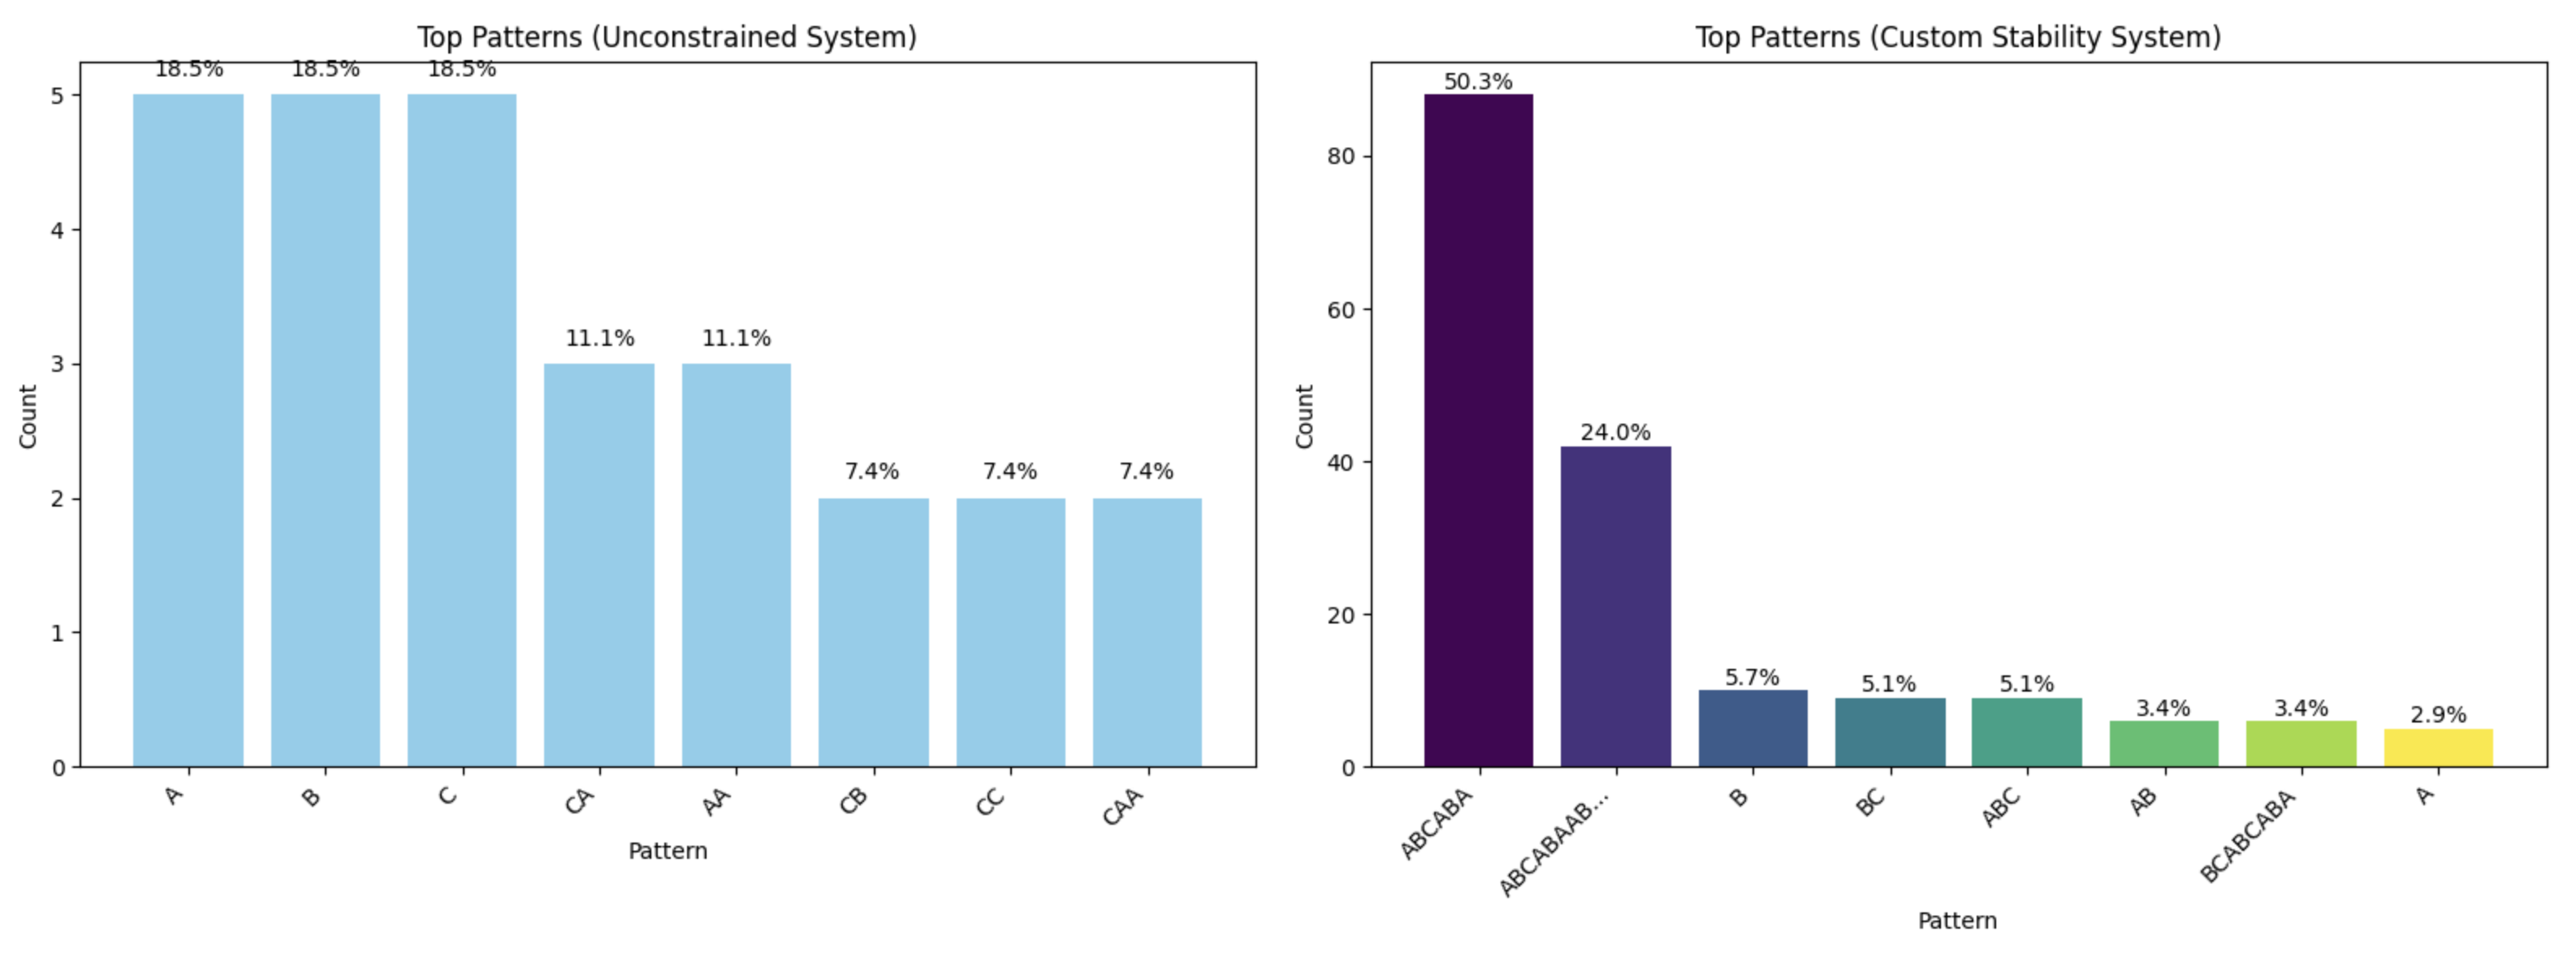
\includegraphics[width=1\textwidth]{SDA-concat-patterns.png}
    \caption{Pattern distribution in the SDA system with concatenation. A small set of high-stability motifs dominate the population, while other patterns are nearly absent.}
    \label{fig:concat-patterns}
\end{figure}

\begin{figure}[H]
    \centering
    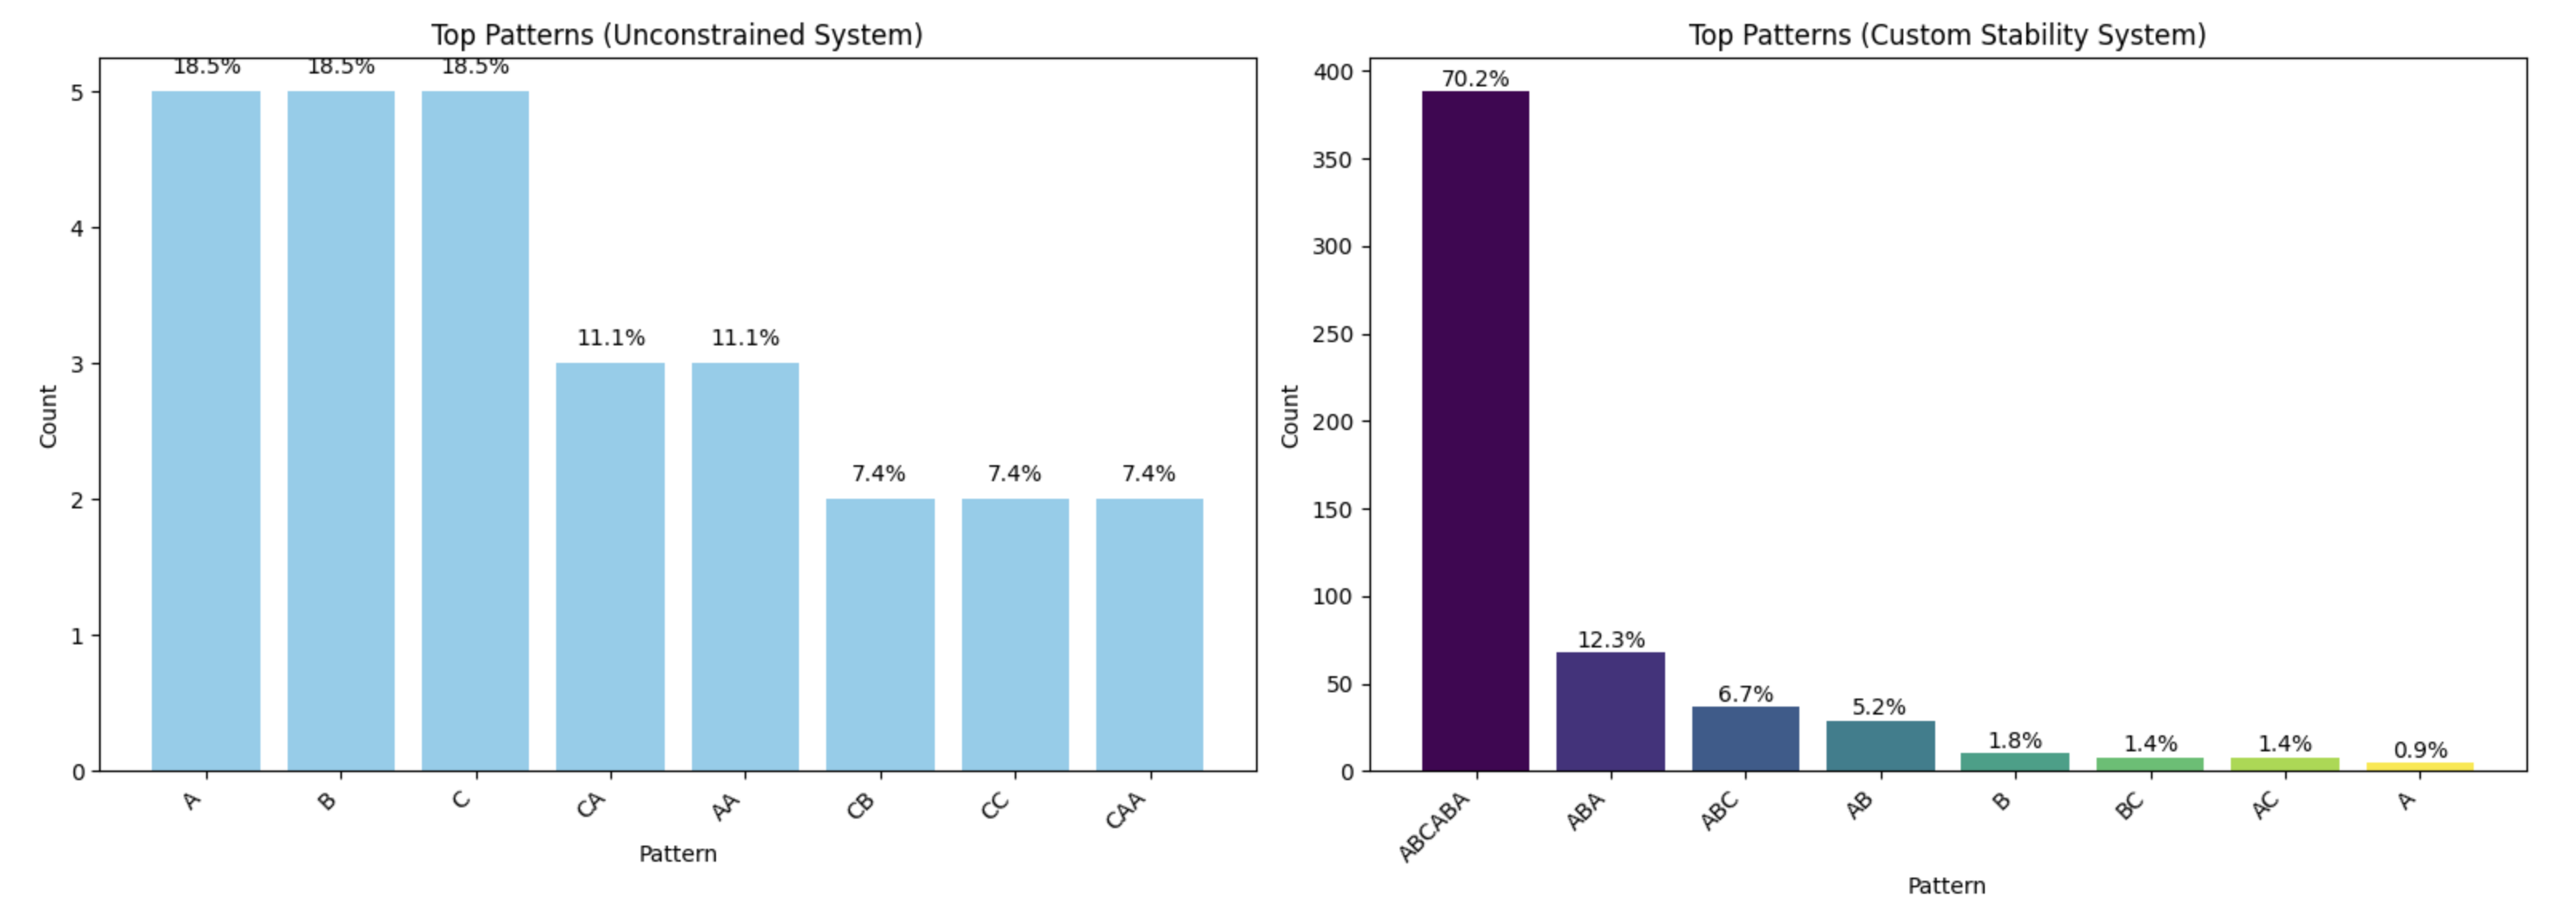
\includegraphics[width=1\textwidth]{SDA-GA-patterns.png}
    \caption{Pattern distribution in the generalized SDA/GA system with recombination. Stable motifs dominate as in the pure SDA case, but a broader tail of low-frequency variants persists due to recombination.}
    \label{fig:ga-patterns}
\end{figure}

Turning to entropy dynamics, both systems show clear reduction in Shannon entropy ($H(P_t) = - \sum_{p \in P} P_t(p) \log_2 P_t(p)$) of
the pattern distribution at generation t measured in bits relative to the unconstrained baseline, confirming the emergence of order and the presence of selection pressure (Figures~\ref{fig:concat-entropy},~\ref{fig:ga-entropy}). Importantly, this occurs without any explicit fitness-proportional selection rule in the algorithm: roulette-wheel selection emerges intrinsically from persistence, since patterns with longer lifetimes are overrepresented and thus more likely to be sampled for further interactions.

In the concatenation-based SDA, while the average entropy goes down from $\sim6$ bits to $\sim4$ bits, its trajectories often exhibit oscillations. These arise because concatenation tends to build large, synchronized cohorts of similar long motifs, which expire at nearly the same time. When such a cohort collapses, replenished base elements briefly increase diversity and entropy before new dominant motifs emerge, creating a characteristic boom–bust cycle. In contrast, in the recombination-based SDA/GA, entropy decreases more smoothly to $\sim3$ bits without oscillations. Recombination produces mosaic offspring with staggered lifetimes, desynchronizing expirations and damping collective turnover. The result is a more monotonic entropy collapse toward a skewed distribution anchored by stable motifs.

\begin{figure}[H]
    \centering
    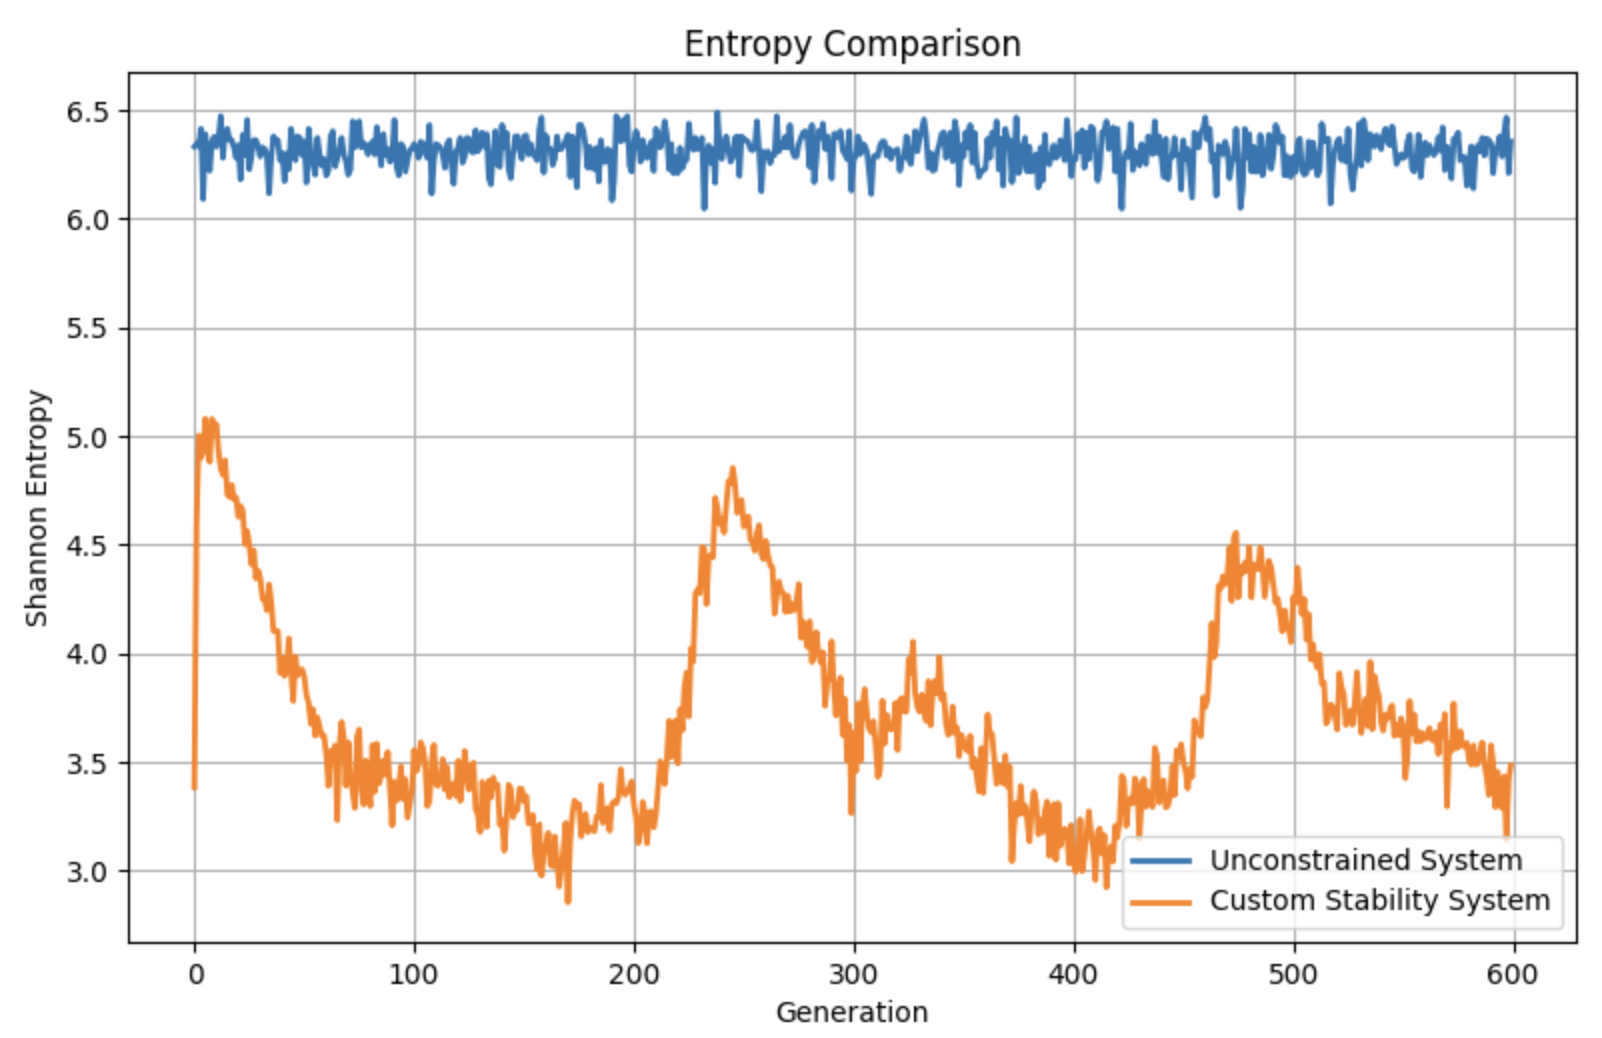
\includegraphics[width=0.8\textwidth]{SDA-concat-entropy.png}
    \caption{Entropy dynamics in the concatenation-based SDA system. Entropy decreases overall but exhibits oscillatory boom–bust cycles due to synchronized expiration of long motifs.}
    \label{fig:concat-entropy}
\end{figure}

\begin{figure}[H]
    \centering
    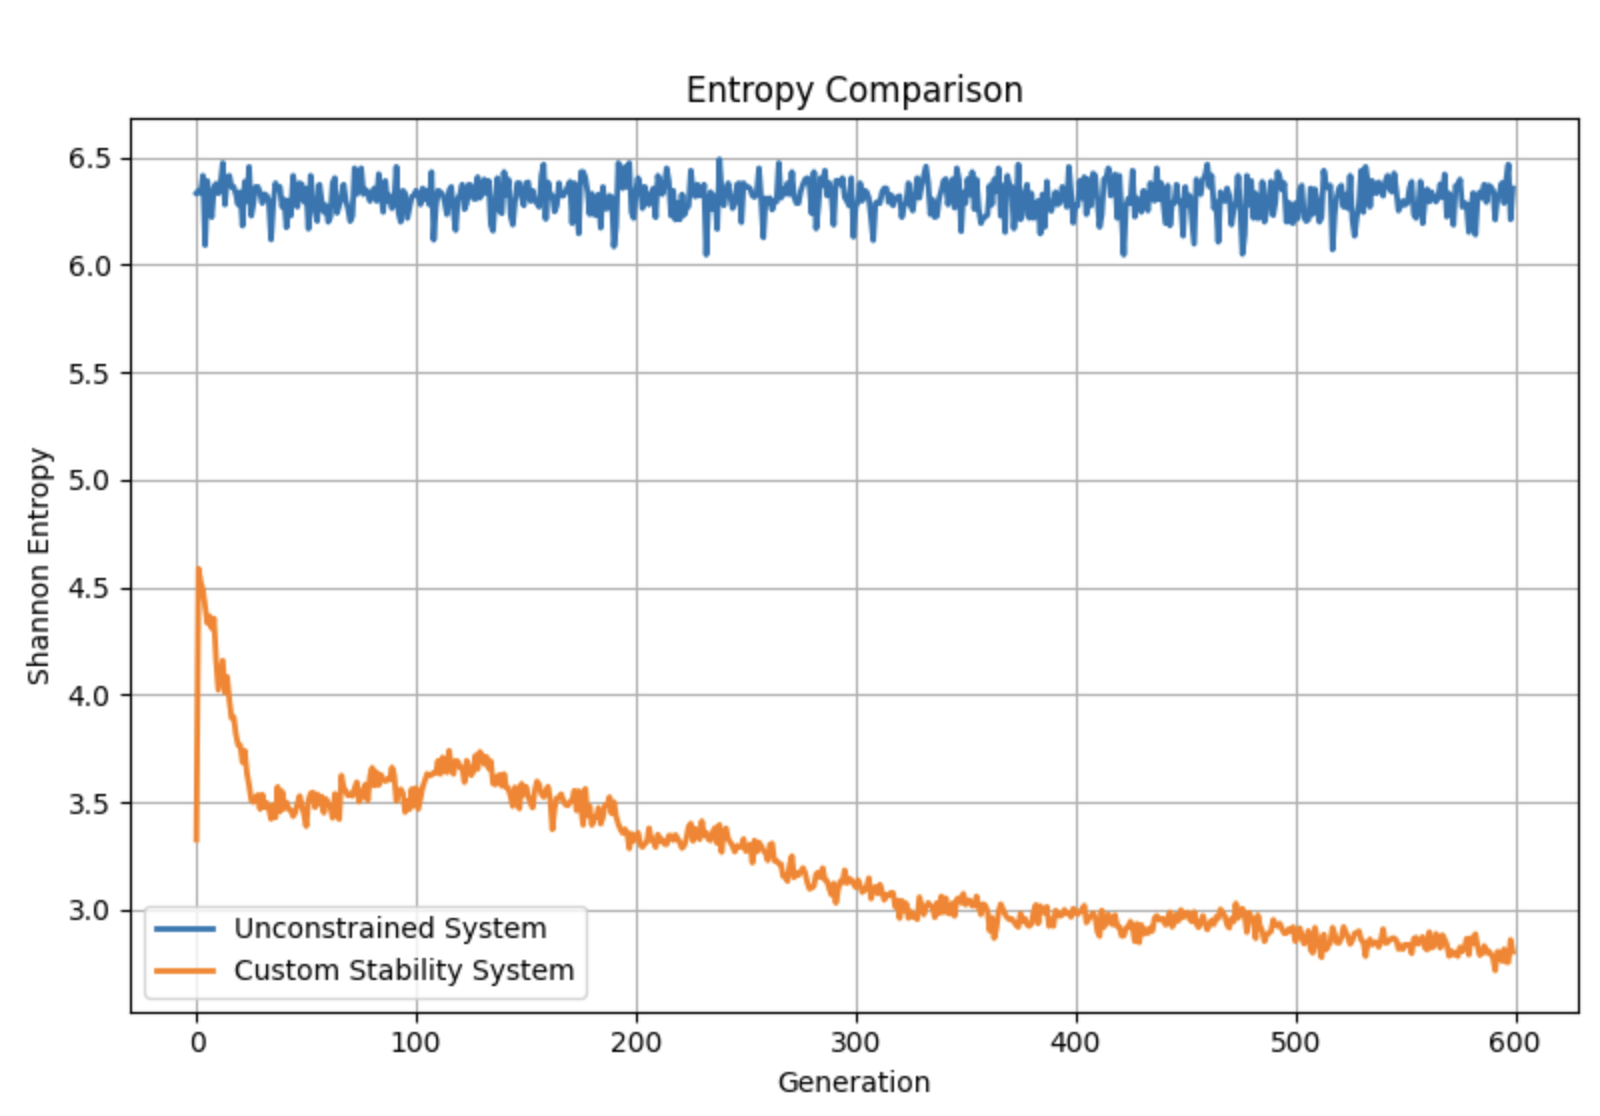
\includegraphics[width=0.8\textwidth]{SDA-GA-entropy.png}
    \caption{Entropy dynamics in the recombination-based SDA/GA system. Entropy decreases smoothly without oscillations, as recombination desynchronizes expirations.}
    \label{fig:ga-entropy}
\end{figure}

Together, these results demonstrate that stability-driven assembly robustly yields emergent selection pressure and entropy reduction under both concatenation and recombination operators. The choice of interaction operator primarily shapes the dynamical form of convergence: oscillatory cycles under concatenation versus smooth decline under recombination.

\begin{figure}[H]
    \centering
    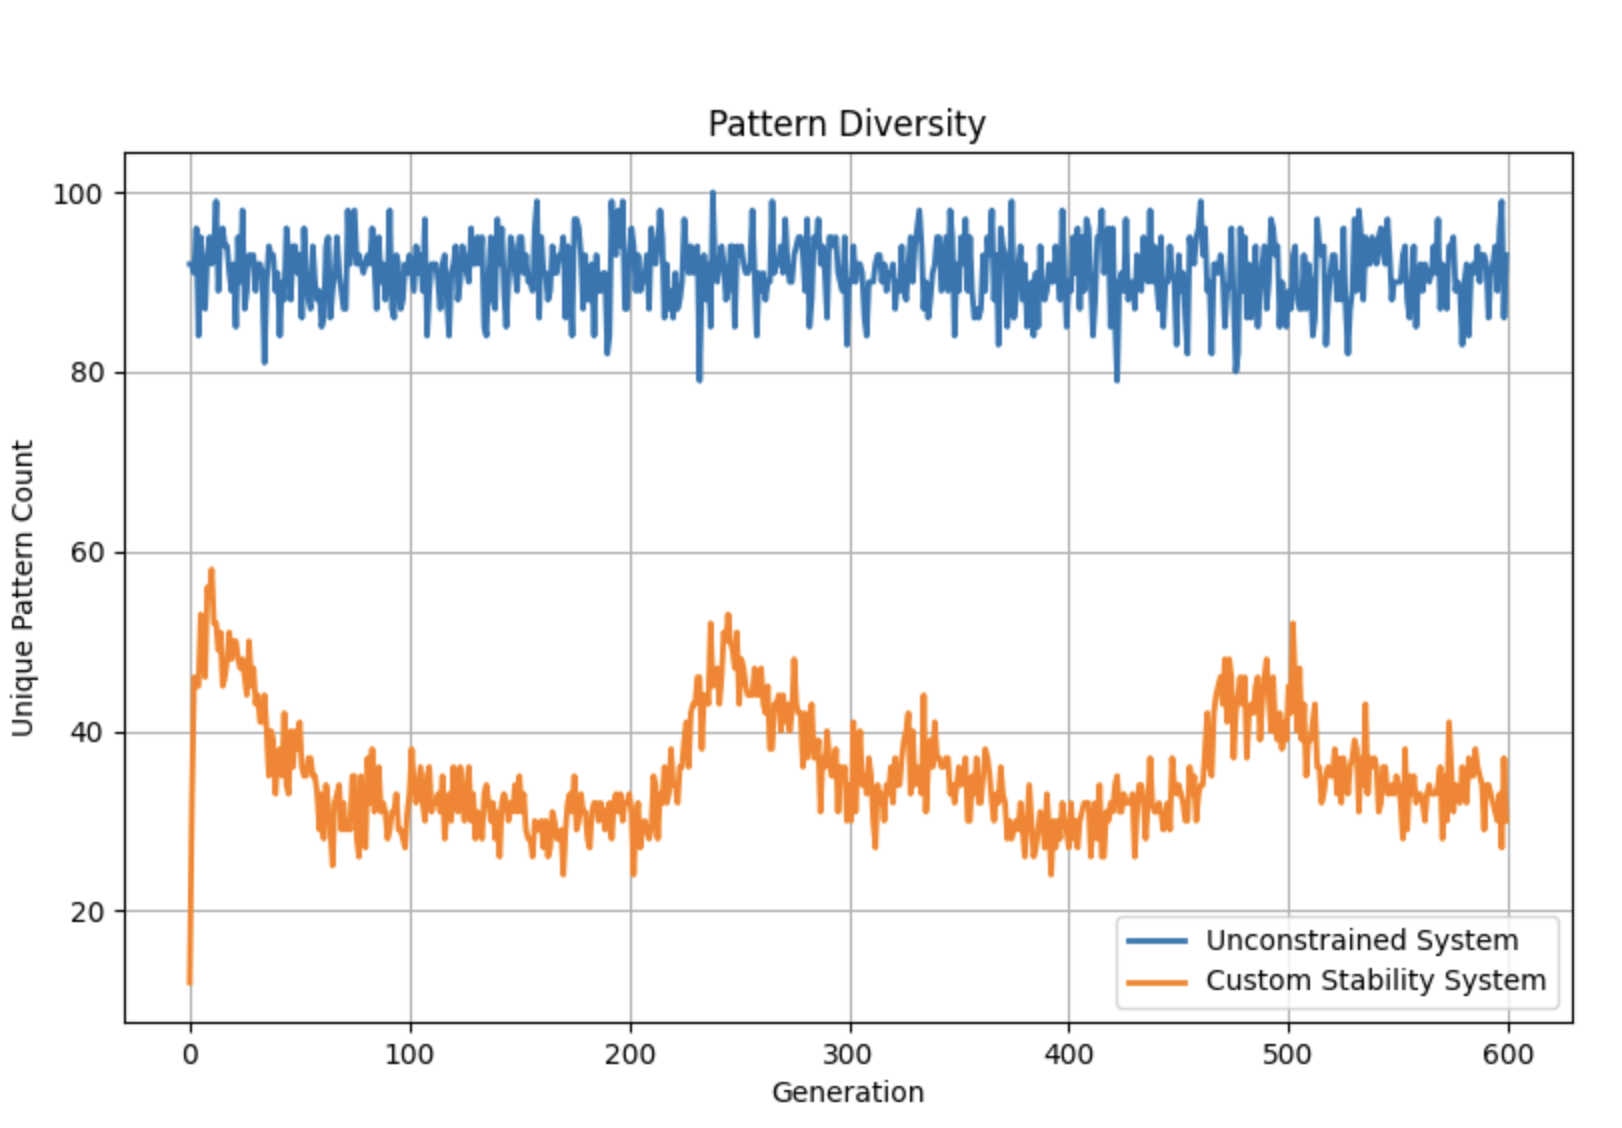
\includegraphics[width=0.75\textwidth]{SDA-concat-diversity.png}
    \caption{Pattern diversity in the concatenation-based SDA. Diversity oscillates in tandem with entropy, reflecting boom--bust cycles of synchronized motif turnover.}
    \label{fig:concat-diversity}
\end{figure}

\begin{figure}[H]
    \centering
    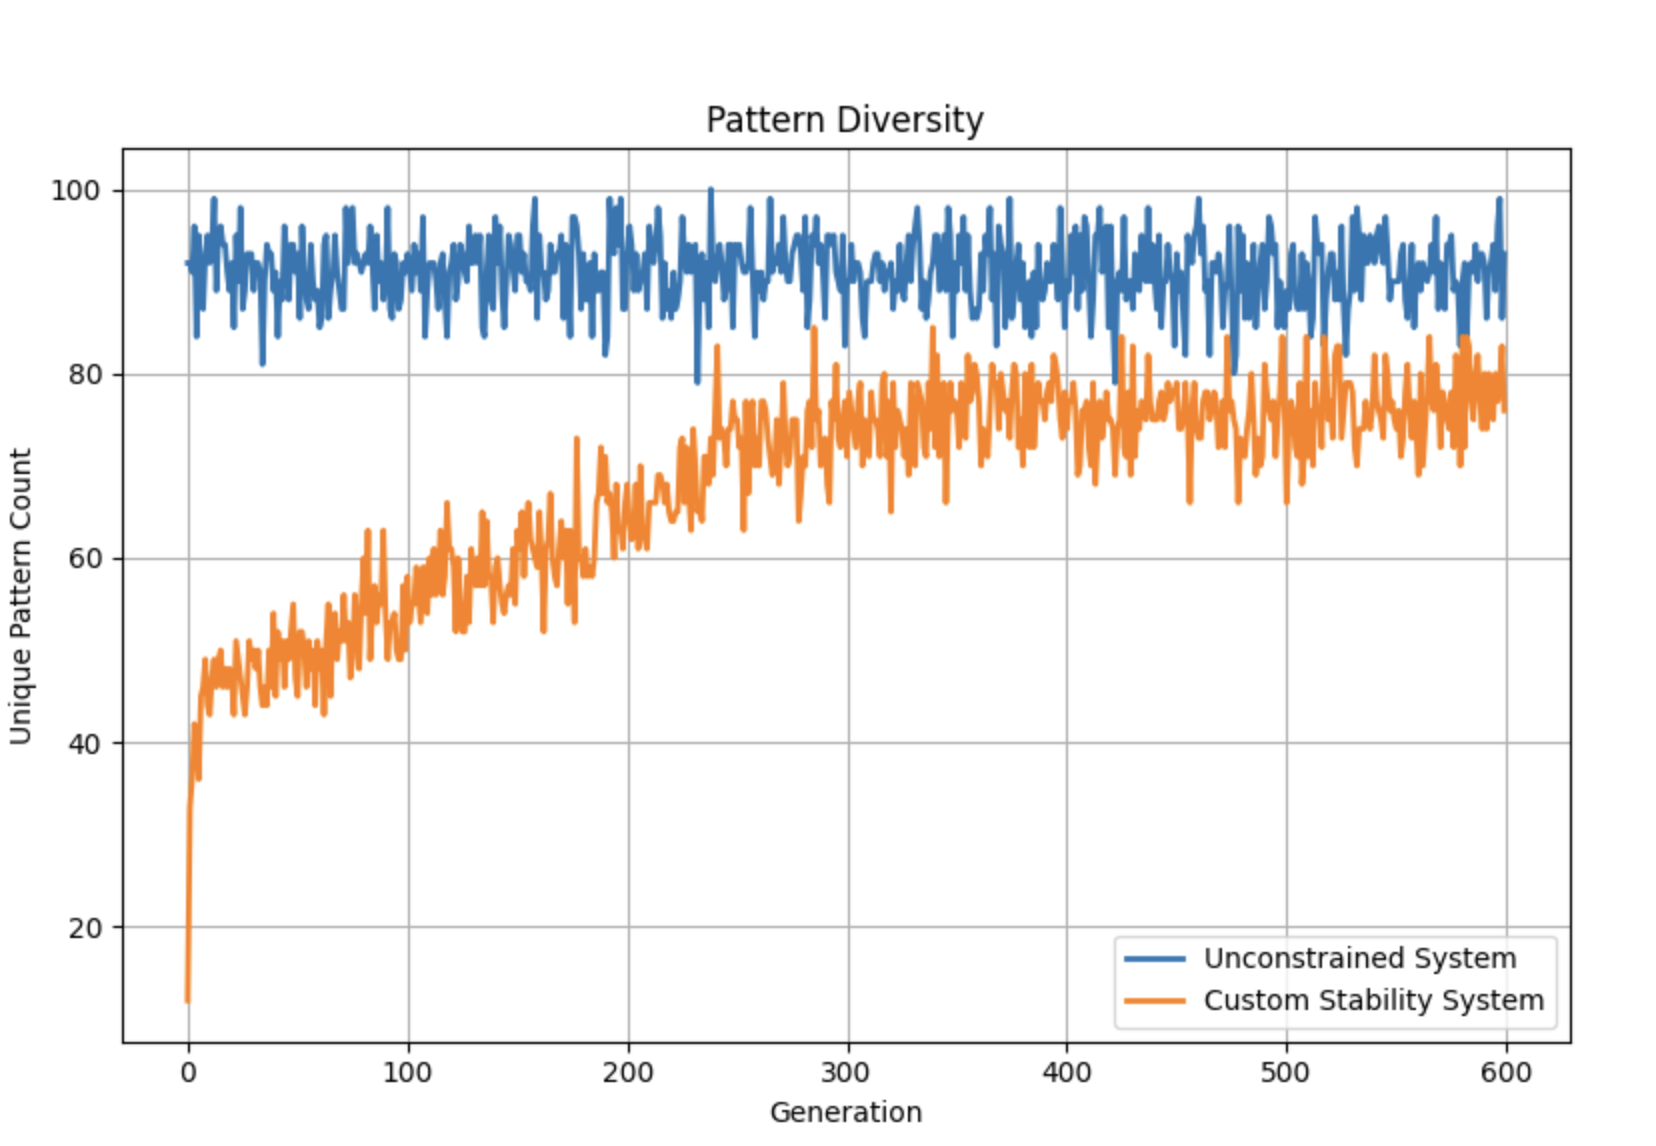
\includegraphics[width=0.75\textwidth]{SDA-GA-diversity.png}
    \caption{Pattern diversity in the recombination-based SDA/GA. Diversity steadily rises toward unconstrained levels, indicating continuous generation of low-frequency variants.}
    \label{fig:ga-diversity}
\end{figure}

The unique pattern diversity results in Figures~\ref{fig:concat-diversity} and~\ref{fig:ga-diversity} highlight the exploration--exploitation tradeoff. 
In concatenation-based SDA, exploration of pattern space is intermittent: 
diversity rises when base elements re-enter, then collapses as a dominant 
motif takes over, producing oscillatory boom--bust dynamics. In contrast, 
recombination-based SDA/GA sustains a broader exploration of the space, 
with diversity approaching unconstrained levels even though entropy 
collapses. Most of these additional patterns remain low-probability, but 
their presence shows that recombination and mutation inject continuous 
novelty. Thus, SDA/GA combines strong exploitation of stable motifs with 
ongoing exploration of alternatives---a hallmark of genetic algorithms---all 
emerging naturally without an explicit fitness function.


We also tested the effect of introducing low-probability, single-site mutations during recombination. 
These mutations serve as a simple model of stochastic perturbations such as copying errors or 
diffusion events. As expected, mutation did not qualitatively alter the dynamics: entropy still 
collapsed and high-stability motifs remained dominant. The principal effect was a modest increase 
in diversity, with rare variants persisting slightly longer. Importantly, mutation did not reintroduce 
oscillations into the GA case nor disrupt the overall reduction in entropy, confirming that the 
emergent selection mechanism is robust to stochastic noise.

\section{Genetic Algorithms and Natural Genetic Algorithms}

The study of genetic algorithms (GAs) has a long history in computer science and optimization. 
Holland’s foundational work \cite{holland1975adaptation} introduced the idea of using crossover, 
mutation, and selection to evolve solutions to computational problems. Later, Goldberg 
\cite{goldberg1989genetic} popularized and formalized GAs as practical optimization tools, 
particularly for engineering and combinatorial search. Building on this tradition, Koza 
\cite{koza1992genetic} extended the paradigm to genetic programming (GP), in which whole 
program trees rather than fixed-length strings evolve under crossover and mutation. GP has 
been especially influential in symbolic regression and in evolving nontrivial structures such 
as circuits, strategies, and controllers.

In all of these approaches, the defining feature of a GA or GP is that the \emph{fitness function} 
is externally specified by the programmer. The GA loop evaluates each candidate solution, assigns 
a fitness value, and uses that fitness to bias the sampling of parents. Whether the goal is 
minimizing error in a regression task or maximizing throughput in a design problem, the selective 
pressure is supplied by the problem designer.


By contrast, in a Stability-Driven Assembly (SDA) system the selection mechanism is not externally 
programmed but emerges intrinsically from persistence. Each pattern has a stability $S(p)$, 
which determines how long it remains in the population. Patterns with higher stability survive 
longer, become more frequent, and are therefore more likely to be sampled for further 
recombination. This effectively implements a roulette-wheel selection scheme without explicitly 
specifying one in the algorithm.

In simple string models, the stability function $S$ may be assigned by hand to highlight specific 
motifs, which makes the dynamics easy to visualize. However, in real-world contexts the stability 
function is determined by the environment itself. In chemistry, for example, molecular stability 
arises from thermodynamics, kinetics, and reaction constraints. In biology, environmental conditions 
determine whether a sequence or structure persists. Thus, while a traditional GA requires the 
programmer to provide an explicit fitness function, a natural GA---as instantiated by SDA---derives 
its fitness measure from the environment. This distinction is crucial for interpreting SDA not 
merely as an algorithmic metaphor but as a model of how nature itself performs search and selection.

Classical GA uses an explicit programmer-supplied fitness function $f$ to bias selection. 
In SDA, there is no explicit selection operator: each pattern $p$ receives a stability 
$S(p)$ that sets its expiration time $t_{\exp}(p)=t+S(p)$. Patterns with larger $S(p)$ 
persist longer and are therefore sampled more often for recombination, yielding 
fitness-proportional selection \emph{in expectation} without computing $f$. 
For toy strings, $S$ may be assigned by design; for realistic chemistry, $S$ is determined 
by the environment (valence/duet–octet satisfaction, sterics, thermodynamics, kinetics, 
reactor residence time). Thus, SDA \emph{builds fitness into persistence}, whereas GA 
\emph{supplies fitness explicitly}.

One of the most widely known illustrations of genetic algorithms is Dawkins’ “weasel” program \cite{dawkins1986blind}. In this example, random sequences of characters evolve toward a fixed target phrase (“METHINKS IT IS LIKE A WEASEL”) through repeated variation and selection. The program demonstrates how cumulative selection can rapidly find a solution compared to random search, but it does so by imposing an externally defined goal and fitness criterion. While useful as a teaching tool, the weasel program exemplifies target-driven search, in contrast to the open-ended dynamics we seek to model here.

A closer analogy to SDA than Dawkins’ “weasel” is jazz improvisation \cite{{adler2025jazz}}. In jazz, musicians explore an open-ended space of notes and motifs without a fixed target. Motifs that resonate are repeated, developed, exchanged and and recombined, while those that do not fit disappear. Over time, structure and themes emerge from this stochastic yet biased search. In SDA, stochastic interactions explore assembly space, persistence bias favors stable motifs, and new motifs accumulate without any pre-specified goal. Both processes are creative in the same sense: they discover what works by letting persistence guide variation. This analogy highlights why SDA differs fundamentally from target-driven search models, illustrating how novelty and information can emerge from feedback between persistence and stochastic exploration.

\section{Application to Organic Chemistry}

The abstract SDA/GA framework can be instantiated in chemical symbol space to model 
the spontaneous evolution of molecular populations. In this setting, the base elements 
$E$ are drawn from the atomic alphabet (C, O, N, H, etc.), and the interaction operator 
$\oplus$ is instantiated as recombination and mutation of molecular fragments. 

Genetic algorithms and genetic programming have long been applied in chemistry and 
cheminformatics, particularly for de novo molecular design and drug discovery 
\cite{brown2004ga,lewis1998gp,jensen2019ga,yoshikawa2018ga}. These approaches typically 
represent molecules as graphs or strings and apply crossover and mutation operators 
guided by an externally defined fitness function, such as binding affinity, 
drug-likeness, or synthetic accessibility. Fink and Reymond’s construction of the 
GDB-11 database \cite{fink2007gdb11} demonstrated the sheer size of chemically valid 
search space, generating over 26 million molecules with up to eleven atoms and over 
110 million stereoisomers. Yet only a minute fraction of these compounds occur in 
public databases, underscoring both the vastness of chemical possibility and the 
impracticality of uniform or ergodic search. This observation motivates the use of 
search strategies that inherently bias exploration toward persistent and chemically 
stable motifs. Whereas traditional GA/GP methods rely on explicit, human-specified 
fitness functions to impose such bias, the SDA/GA framework does so intrinsically by 
embedding stability into persistence, allowing selection pressure to emerge directly 
from environmental constraints such as valence rules, steric feasibility, and 
thermodynamics.

It is important to emphasize that the present work is not aimed at drug discovery 
or molecular optimization applications, which have been the traditional focus of 
genetic algorithms and genetic programming in chemistry. Instead, our goal is 
conceptual: to hypothesize how nature itself may have acted as a “natural genetic 
algorithm,” using stability-driven persistence as the implicit fitness function to 
non-ergodically explore the astronomical chemical space revealed by studies such 
as GDB-11. Within this perspective, the emergence of a biosphere can be viewed as 
the outcome of stability-biased sampling: persistent motifs accumulate, dominate, 
and recombine, gradually transforming an unconstrained chemical universe into a 
structured, evolving system.

The mapping in Table~\ref{tab:chem-sda-operators} illustrates how common classes of organic reactions can be interpreted within the SDA/GA framework. Substitution, reduction, and oxidation reactions all correspond to \textit{mutations}, since they alter functional groups while preserving the underlying scaffold. Addition reactions may play either role: the attachment of a small atom or group is best regarded as mutation, whereas the joining of two larger fragments constitutes recombination.  

Acid--base reactions are a particularly simple but important form of mutation. Protonation and deprotonation cycles alter charge states and stability without changing the covalent backbone, yet they have profound effects on persistence in different environments. Similarly, isomerization represents a mutational step in which the connectivity or geometry is reshuffled, sometimes uncovering stability differences that bias persistence even though no atoms are gained or lost.  

Polymerization, including peptide bond formation, provides a canonical example of recombination. Here, motifs link through edge-biased joining to form larger assemblies. Once formed, such chains introduce new levels of persistence and complexity, laying the groundwork for the higher rungs of the evolutionary ladder. Fragmentation and dissociation serve as the inverse of recombination, redistributing persistence across smaller motifs.  

This mapping shows that the SDA operators of mutation and recombination are not abstract inventions but correspond directly to well-established categories of chemical reactivity. This correspondence grounds the abstraction in chemical reality and illustrates how stability-driven selection could operate in real chemical networks without requiring additional operators beyond those already available to organic chemistry.


\begin{table}[H]
\caption{Mapping of classical organic reactions to SDA operators.\label{tab:chem-sda-operators}}
\begin{adjustwidth}{-\extralength}{0cm}
\begin{tabularx}{\fulllength}{XXX}
\toprule
\textbf{Reaction Type} & \textbf{Chemical Example} & \textbf{SDA Operator Analogy} \\
\midrule
Substitution & 
Aldehyde $\to$ imine (R--CHO + R'NH$_2$) &
Mutation: substituent replaced while scaffold persists. \\
\midrule
Reduction & 
Aldehyde $\to$ alcohol (R--CHO $\to$ R--CH$_2$OH) &
Mutation: functional group altered by gain of H atoms. \\
\midrule
Oxidation & 
Aldehyde $\to$ carboxylic acid (R--CHO $\to$ R--COOH) &
Mutation: functional group altered by increase in bond order/O atoms. \\
\midrule
Addition & 
Nucleophilic addition to carbonyl (R--C=O + HX $\to$ R--C(OH)X) &
Recombination if a whole fragment attaches; mutation if a small group adds. \\
\midrule
Acid--Base & 
Amines or carboxylic acids (R--NH$_2$ + H$^+$ $\leftrightarrow$ R--NH$_3^+$) &
Mutation: reversible change in protonation state or charge. \\
\midrule
Polymerization / Peptide Formation & 
Amino acids $\to$ peptide chains &
Recombination of motifs; edge-biased joining. \\
\midrule
Isomerization & 
Keto--enol tautomerism, cis/trans isomers &
Mutation: rearrangement of structure without adding/removing parts. \\
\midrule
Fragmentation / Dissociation & 
Ester hydrolysis (R--COOR' $\to$ R--COOH + R'OH) &
Inverse of recombination; persistence split across products. \\
\bottomrule
\end{tabularx}
\end{adjustwidth}
\end{table}

In classical chemistry, these transformations are usually presented as synthesis pathways, each requiring specific reagents, catalysts, and conditions. In contrast, the SDA framework abstracts away from mechanistic detail to emphasize population-level dynamics: regardless of the stepwise route, persistence and recombination biases determine which motifs accumulate. Thus, SDA complements the traditional synthesis perspective by revealing how macro-level selection effects emerge from the distribution of possible transformations.


The abstract operators in Table~\ref{tab:chem-sda-operators} can be illustrated with specific examples. 
Figure~\ref{fig:mutation-recombination}a shows a \textit{mutation} event, within our
simulation framework, in which ethanol CCO is converted to isopropanol CC(C)O, 
a local substitution that preserves the scaffold while altering stability. 
Figure~\ref{fig:mutation-recombination}b demonstrates a \textit{recombination} event: 
COCCO and CCOC(=O)C combine to produce CCOC (dimethyl ether). 
These cases exemplify how mutations correspond to local functional changes, 
while recombinations join fragments from different parents to generate novel motifs. 


\begin{figure}[H]
\begin{adjustwidth}{-\extralength}{0cm}
\centering
\subfloat[\centering Mutation]{
  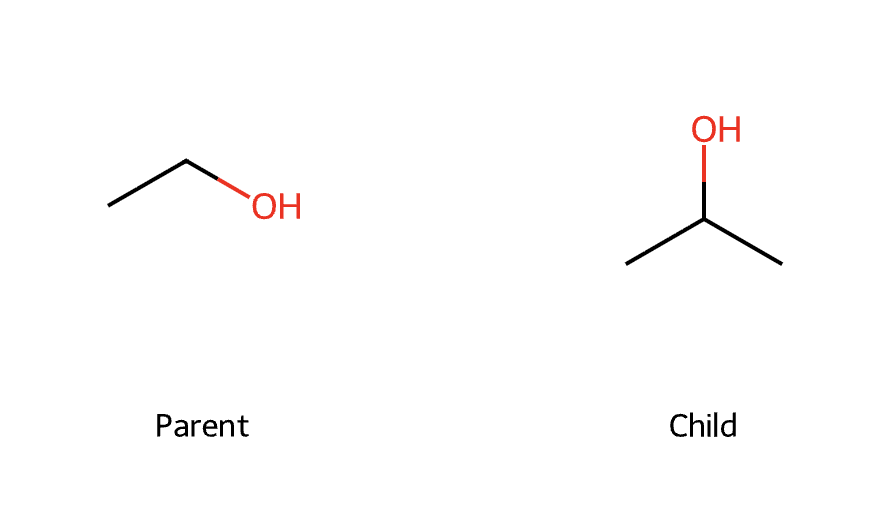
\includegraphics[width=5cm]{mutation_example.png}}
\hspace{0.4cm}
\subfloat[\centering Recombination]{
  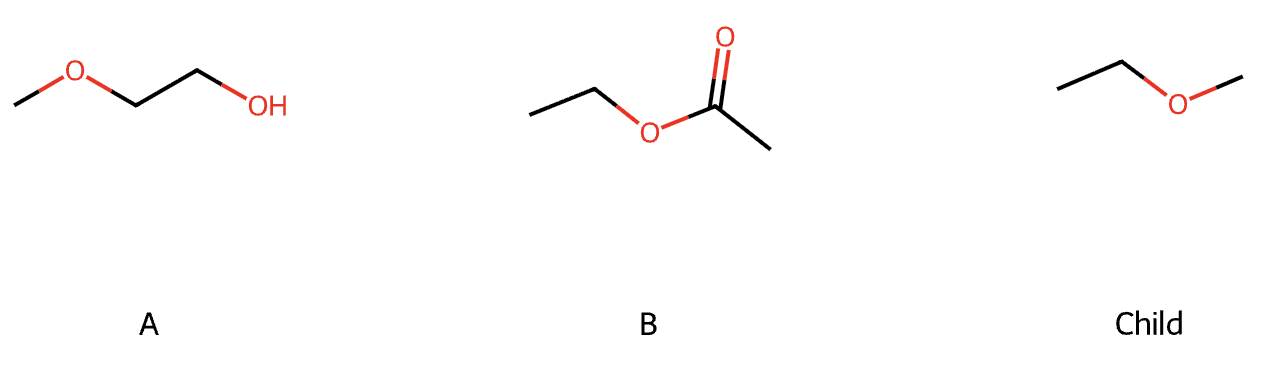
\includegraphics[width=7cm]{recombination_example.png}}
\end{adjustwidth}
\caption{Examples of SDA operators in chemical form. (\textbf{a}) Mutation: ethanol CCO $\to$ isopropanol CC(C)O. 
(\textbf{b}) Recombination: COCCO + CCOC(=O)C $\to$ CCOC.}
\label{fig:mutation-recombination}
\end{figure}

Note that some of these mutations and recombinations do not correspond to single-step reactions in real chemistry and, in practice, may require multistep synthesis pathways, catalysts, or additional energy inputs. In the SDA framework, however, they are abstracted into single operators in order to isolate the role of persistence bias and population dynamics, leaving mechanistic details to future, more chemically specific implementations.


\subsection{Patterns as Molecules}
Patterns correspond to molecules represented in SMILES notation. Recombination is implemented 
using BRICS fragmentation and reassembly, ensuring that new molecules respect basic valence 
rules and avoid chemically implausible bonds. Mutation is modeled as single-site perturbations, 
analogous to copying errors or diffusion-induced reactions, again constrained by chemical 
plausibility.

\subsection{Stability as Persistence}
In the chemical domain, the stability function $S(p)$ is determined by the environment rather 
than by the algorithm designer. For organic molecules, persistence may reflect compliance with 
the octet rule, avoidance of strained substructures, thermodynamic feasibility, or kinetic 
barriers to decay. In practice, we operationalize $S(p)$ using fast cheminformatics heuristics 
(RDKit valence checks, BRICS rules) that enforce plausible structures. More detailed models 
could extend $S(p)$ to incorporate semiempirical energy estimates or experimentally derived 
lifetimes.

\subsection{Simulation Examples}
Applying the SDA/GA procedure to organic fragments yields results analogous to the string 
experiments. High-stability motifs dominate the population, while recombination continually 
generates low-frequency variants, maintaining a fat-tailed distribution of molecules. Entropy 
collapses as selection pressure drives convergence, yet diversity remains higher under 
recombination than under concatenation, reflecting ongoing exploration of chemical space. 
These dynamics mirror nature’s own exploration of chemical possibility: vast combinatorial 
search space is sampled non-ergodically, biased toward persistent structures.

\subsection{Interpretation}
This chemical instantiation highlights the central claim of SDA: selection emerges not from 
an externally defined fitness function, but from persistence. In GA terms, fitness is 
\emph{calculated} by the environment. In practice, octet completion, steric constraints, and 
reaction kinetics determine which molecules last long enough to be sampled again. Thus, the 
SDA/GA framework offers a naturalistic model of molecular evolution, one that unifies symbolic 
cheminformatics with dynamical systems principles.

\section{Chemical SDA/GA Simulation}

\subsection{Methods}

To extend the symbolic SDA/GA framework into the chemical domain, we reused the same minimal simulation loop with only two modifications. First, symbolic string elements were replaced with SMILES fragments drawn from a small set of base compounds (e.g., \texttt{C}, \texttt{CC}, \texttt{O}, \texttt{CO}, etc.), representing a rudimentary pool of prebiotic building blocks. Second, instead of assigning fixed stability values, we introduced a callable stability function $S(p)$ that estimates the persistence of a compound from molecular features. For demonstration purposes, this was implemented as a function of heavy atom count with heuristic boosts for chemically plausible motifs such as carboxylates, esters, and amides. In this formulation, fitness is not supplied externally, but arises from chemical plausibility as encoded in stability, thereby aligning with the SDA principle that selection emerges from persistence rather than externally imposed objectives.  

Molecules were represented as SMILES strings and manipulated using the RDKit cheminformatics toolkit \cite{landrum2006rdkit}. Recombination was implemented through BRICS-based fragmentation and reassembly \cite{degen2008art}. Our approach aligns with recent methodological surveys on best practices for genetic algorithms in molecular discovery \cite{janet2023bestpractices}.

All other aspects of the algorithm were left unchanged. As in the symbolic case, base fragments were replenished each generation, new compounds were formed through recombination and mutation using BRICS rules, and expiration times were assigned according to the stability function. This allows the chemical simulation to be understood as a natural extension of symbolic SDA, with only minimal changes distinguishing abstract informational dynamics from physical chemical dynamics.  

\subsection{Results}

We ran chemical SDA simulations for 1000 generations with 200 interactions per generation and a replenishment rate of five. The results reveal how stability-driven persistence produces skewed population structures, motif-level evolution, and system-wide dynamics that parallel both genetic algorithms (GAs) and ecological systems.  

\begin{figure}[H]
\begin{adjustwidth}{-\extralength}{0cm}
\centering
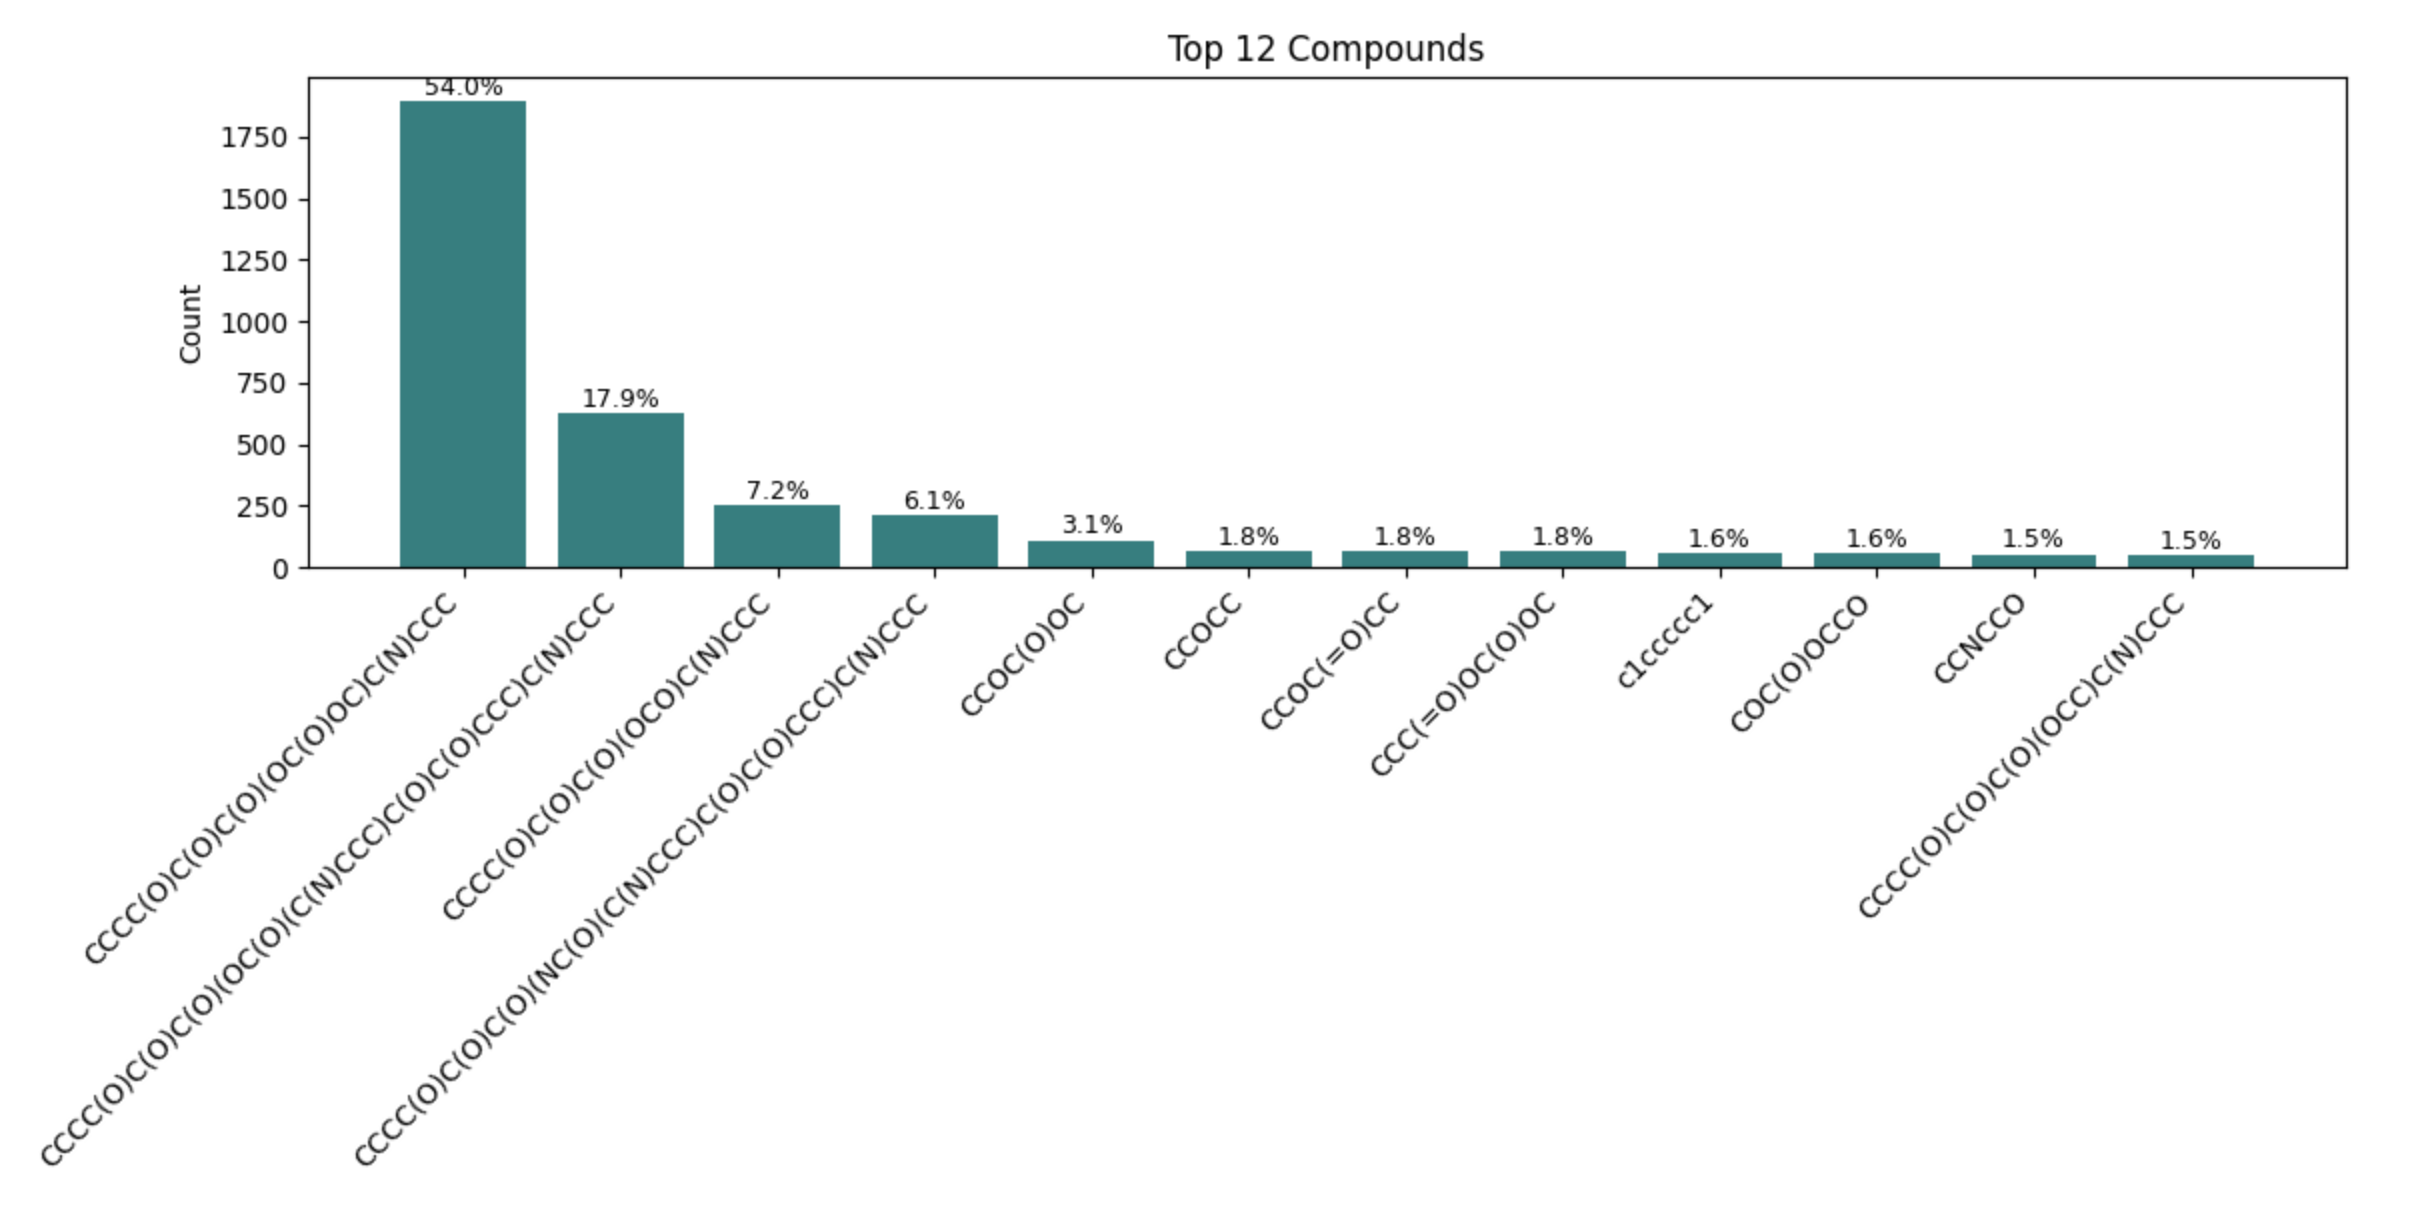
\includegraphics[width=\fulllength]{SDA-chem-hist.png}
\end{adjustwidth}
\caption{Histogram of the twelve most frequent compounds at generation 1000, expressed as counts and percentages. One compound accounts for $\sim$54\% of the population, with the next runner-up at $\sim$18\%.}
\label{fig:chem-compound-hist}
\end{figure}

Figure~\ref{fig:chem-compound-hist} shows the distribution of the twelve most abundant compounds at generation 1000. A single ester-like motif (CCCC(O)C(O)C(O)(OC(O)OC)C(N)CCC) dominates over half of the population ($\sim$54\%), while the second most frequent compound---a recursive oligomer in which the polyol core is extended by an additional C(N)CCC branch---accounts for 18\%. The third and fourth most frequent motifs (at 7\% and 6\%, respectively) are close structural relatives: one retains the O–C(=O)–O ester fragment in a simpler form, while the other incorporates an amide-like NC(O) substitution into the same polyol backbone. Together, these four scaffolds account for over 85\% of the entire pool.

From a GA perspective, this concentration illustrates how roulette-wheel selection emerges naturally from persistence: once a motif survives longer, it contributes disproportionately to the parent pool and thus amplifies its frequency. From a chemical perspective, the winners all share the same polyol–amine backbone, differing only in whether the substituent is ester-like, recursive, or amide-like. In other words, the system converges on a GA schema (the hydroxylated carbon scaffold with an appended amine) and explores variations within that schema, selecting for those with the greatest stability. The dominance of these few compounds therefore reflects both the GA principle of schema preservation and the chemical principle that stable substituents accumulate over evolutionary time.

\begin{figure}[H]
    \begin{adjustwidth}{-\extralength}{0cm}
    \centering
    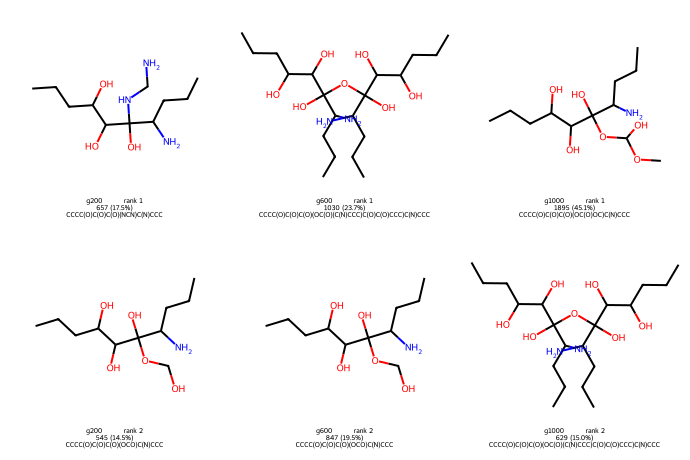
\includegraphics[width=1\textwidth]{SDA-chem-top-evo.png}
    \end{adjustwidth}
    \caption{Evolution of the two top motifs across 200, 600, and 1000 generations. Early competition between NCN- and ester-like variants gives way to long-term fixation of a single stable scaffold.}
    \label{fig:chem-top-evo}
\end{figure}

The trajectories of the two leading motifs are shown in Figure~\ref{fig:chem-top-evo}. At generation 200, the population is split between two scaffolds: an NCN-bearing polyol (17.5\%) and a related ester-like variant (14.5\%). Both share the same hydroxylated carbon backbone with an appended amine chain, differing only in the functional group attached to the central scaffold.  

By generation 600, the competition has shifted. A recursive oligomer that elaborates the NCN branch with an additional polyol–amine extension rises to 23.7\% of the pool, while the ester-like variant persists at 19.5\%. This phase illustrates how SDA dynamics preserve a common schema while exploring more complex recombinants.  

By generation 1000, however, the balance tips decisively. The simpler ester-like scaffold dominates nearly half the population (45.1\%), while the more elaborate recursive oligomer declines to 15.0\%. From a GA perspective, this trajectory illustrates schema competition: multiple variants arise from a shared template, but persistence imbalances weight selection toward those with the most favorable stability. From a chemical perspective, the result shows that moderate substituents (ester-like O–C(=O)–O groups) can outcompete bulkier recursive elaborations, leading to convergence on motifs that maximize both stability and generativity. The outcome thus exemplifies the SDA principle that evolutionary search favors motifs which balance structural richness with long-term persistence.


\begin{figure}[H]
    \centering
    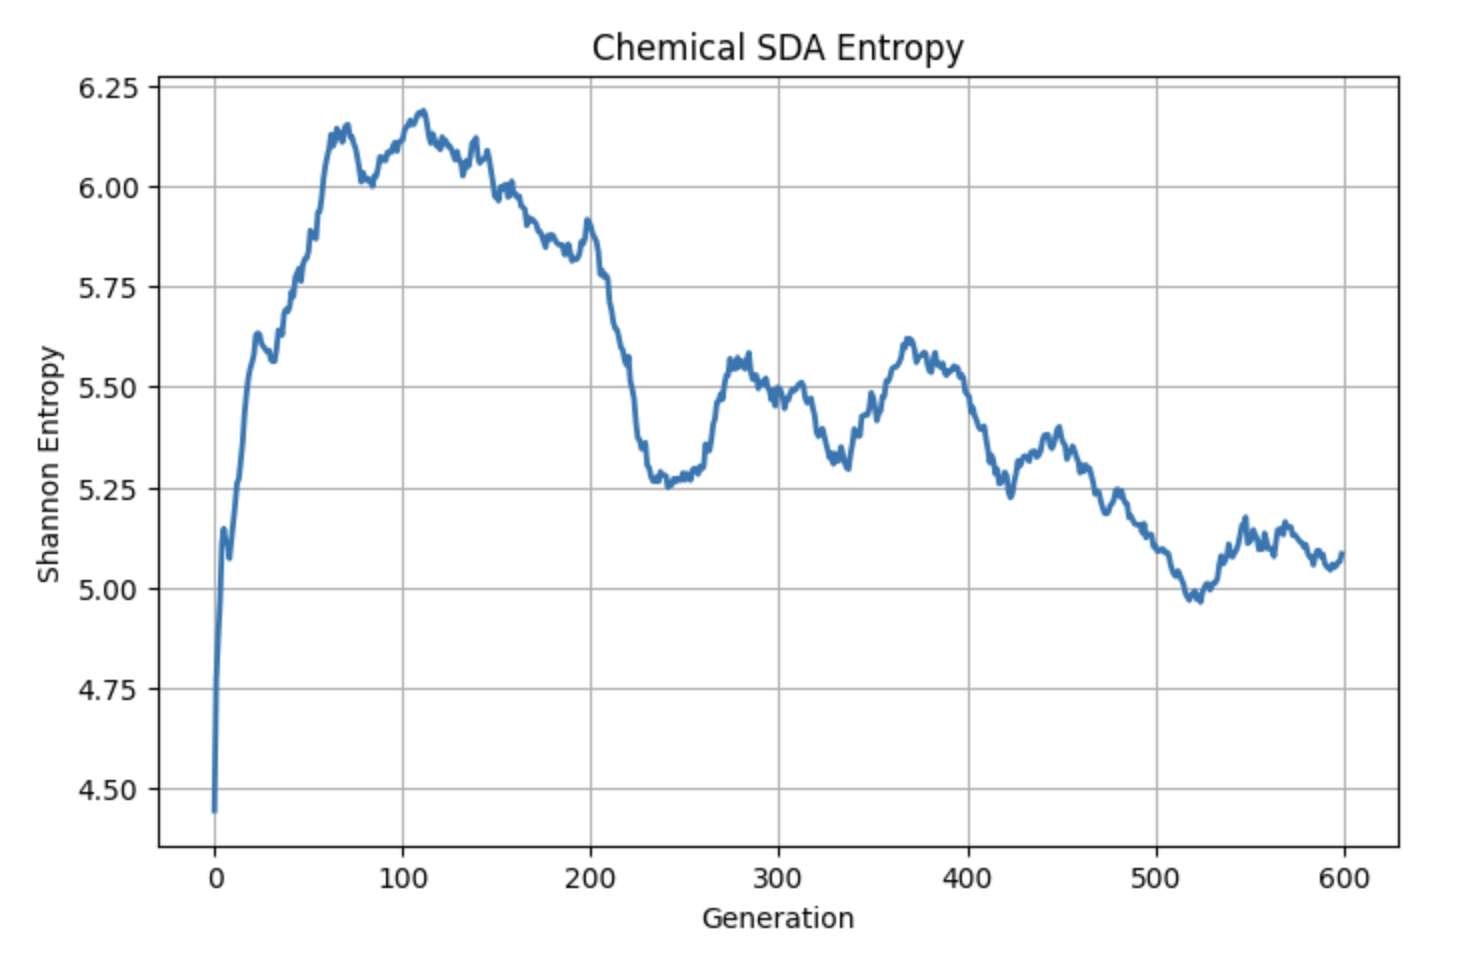
\includegraphics[width=0.7\textwidth]{SDA-chem-entropy.png}
    \caption{Shannon entropy of the chemical SDA population over 1000 generations. Entropy rises sharply as diversity expands, then declines steadily as dominant motifs consolidate.}
    \label{fig:chem-entropy}
\end{figure}

Entropy dynamics, shown in Figure~\ref{fig:chem-entropy}, explain this consolidation. Shannon entropy increases rapidly during early exploration as new compounds are discovered, but after peaking near generation 150--200, it declines monotonically. The decline corresponds to the narrowing of the population into a smaller set of persistent motifs, consistent with selection pruning the search space.  

\begin{figure}[H]
    \centering
    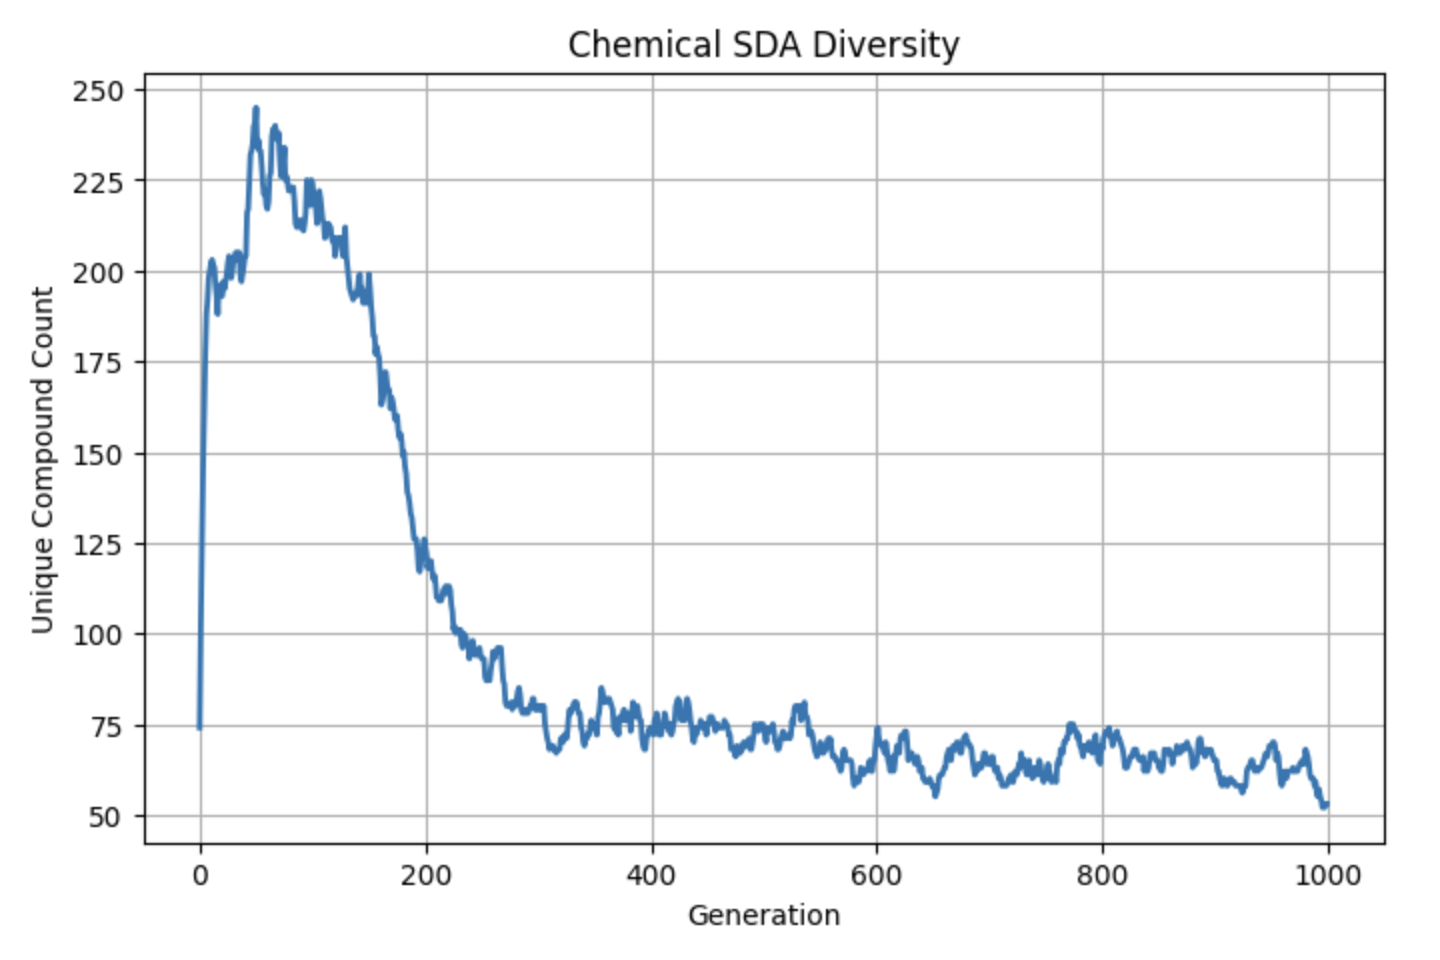
\includegraphics[width=0.7\textwidth]{SDA-chem-diversity.png}
    \caption{Unique compound count over time. Diversity peaks early at over 200 unique species, then collapses to $\sim$50 by the end of the run.}
    \label{fig:chem-diversity}
\end{figure}

Figure~\ref{fig:chem-diversity} shows that diversity follows the same trajectory. The number of distinct compounds rises steeply in the first 100 generations, reaching over 200 species, but collapses thereafter as stability-driven persistence favors only a subset of motifs. By generation 1000, roughly 50 species remain, with the majority of the population concentrated in the top two scaffolds.  

\begin{figure}[H]
    \centering
    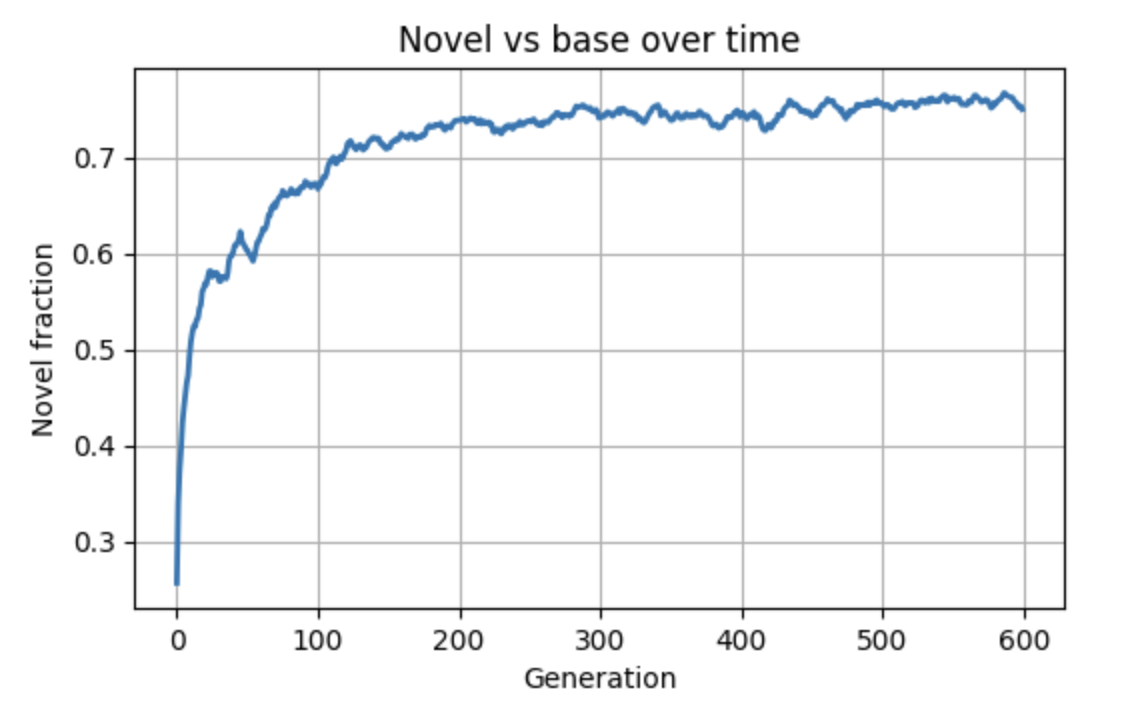
\includegraphics[width=0.7\textwidth]{SDA-chem-novel.png}
    \caption{Fraction of novel compounds (not in the initial fragment pool) over time. Novelty rapidly overtakes the base pool, stabilizing above 80\% of the population.}
    \label{fig:chem-novel}
\end{figure}

Novelty relative to the base fragment set is quantified in Figure~\ref{fig:chem-novel}. The fraction of novel compounds rises steeply and surpasses 80\% by generation 200, remaining stable thereafter. This indicates that evolutionary dynamics are driven by novel recombinations rather than simple recycling of the initial pool. Novelty is thus not transient but sustained, consistent with SDA’s prediction of open-ended exploration.  

\begin{figure}[H]
    \centering
    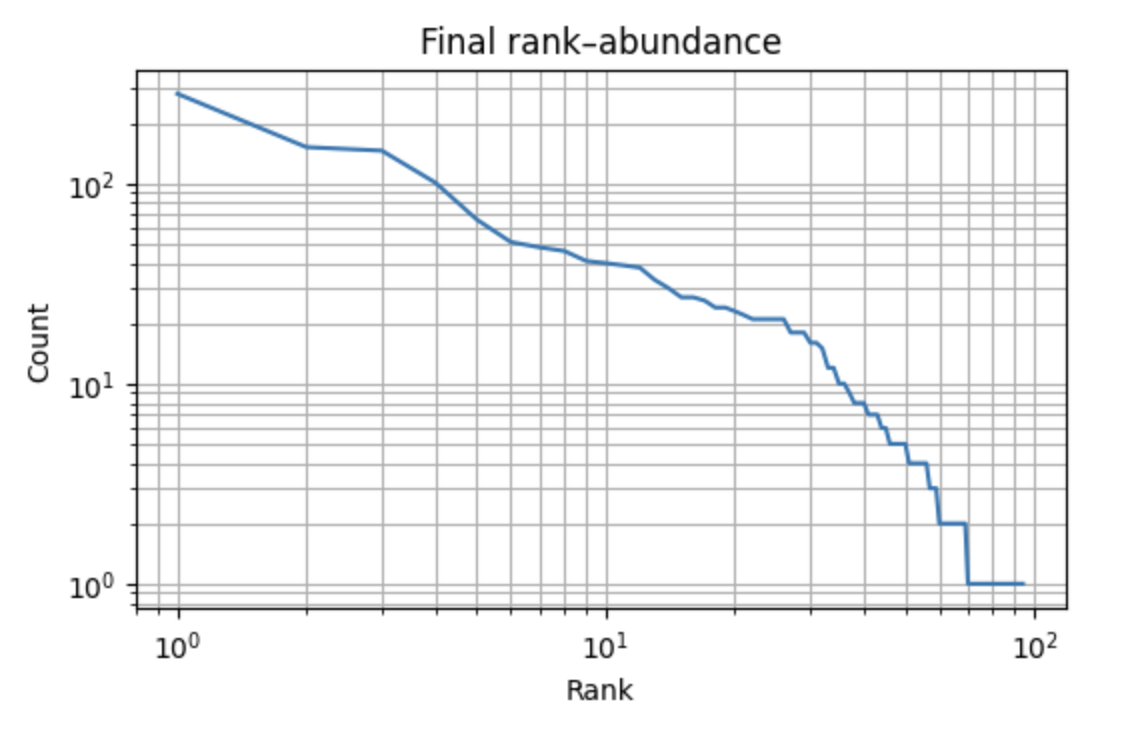
\includegraphics[width=0.7\textwidth]{SDA-chem-rank.png}
    \caption{Rank–abundance distribution of compounds in the final population (log–log scale). A heavy-tailed distribution emerges, with a few highly abundant motifs and many rare species.}
    \label{fig:chem-rank}
\end{figure}

Finally, the rank–abundance distribution in Figure~\ref{fig:chem-rank} shows that the final population adopts a heavy-tailed form. A small number of motifs dominate by orders of magnitude, while a long tail of rare compounds persists at low frequency. This mirrors species-abundance distributions in ecology and demonstrates that SDA naturally produces structured, law-like abundance patterns when applied to chemistry.  

\subsection{Interpretation}

Taken together, these results show that chemical SDA recapitulates the dynamics of a natural GA. Population skew arises spontaneously from persistence imbalances: compounds that survive longer contribute disproportionately to the parent pool, creating effective roulette-wheel selection without an explicit fitness function. This mechanism is evident in the histogram and motif trajectories (Figures~\ref{fig:chem-compound-hist}, \ref{fig:chem-top-evo}), which show oligopolistic dominance and scaffold-level competition.  

System-level traces (Figures~\ref{fig:chem-entropy}--\ref{fig:chem-novel}) explain how this outcome emerges: entropy and diversity expand initially but collapse as selection narrows the space, while novelty remains high as new motifs continually replace base fragments. The final rank–abundance distribution (Figure~\ref{fig:chem-rank}) underscores that these dynamics are not idiosyncratic but follow statistical patterns seen across complex adaptive systems.  

Even with a simplified stability function, the most abundant compounds exhibit chemically plausible motifs such as polyols, esters, and amine substituents. Their persistence is not arbitrary but arises from their ability to withstand turnover in the generative environment. These findings support the SDA hypothesis that stability alone, when coupled with recombination and mutation, can drive both the generation of novelty and the convergence on structured, high-complexity attractors—plausibly capturing the dynamics that underlie prebiotic chemical evolution.  


\subsection{Equilibrium Models versus Selection-Driven Evolution}

It is useful to contrast these results with equilibrium-based analyses such as those presented by MAK. In order to render the governing equations linear and analytically tractable, equilibrium models typically assume constant reaction rates and well-mixed dynamics. This assumption ensures mathematical stability but also suppresses the very features that drive open-ended evolution. With constant rates, all species are treated as equivalent participants in a Markovian flow, and the long-term behavior is dominated by equilibrium concentrations determined by stoichiometry rather than by persistence differentials. In such a setting, once equilibrium is reached, no further directional change occurs.

By contrast, the SDA framework does not impose constant rates or equilibrium conditions. Instead, each compound’s effective lifetime depends on its stability, so that turnover is inherently non-uniform. This creates persistence imbalances: more stable motifs accumulate, while less stable ones vanish, skewing the population distribution and weighting the parent-selection process. As demonstrated in the simulations above, this skew is precisely what produces evolutionary search dynamics. Entropy and diversity expand initially but then collapse as a few stable motifs dominate, novelty is continually generated through recombination, and population abundance assumes a heavy-tailed form reminiscent of ecological communities. None of these features emerge from an equilibrium analysis with constant rates, because such models erase the role of selection in shaping the system’s trajectory.

In short, equilibrium approaches such as MAK characterize the static end-state of a reaction network, whereas SDA captures its inherently evolutionary nature. What appears in equilibrium theory as a steady-state distribution is, in the SDA view, the transient outcome of continual competition, turnover, and selection. This distinction highlights why stability-driven selection is indispensable for understanding how chemical systems can move beyond equilibrium chemistry toward open-ended evolution.


\subsection{Comparison to Supervised Learning and Genetic Programming}  

It is also important to distinguish chemical SDA from supervised learning and from conventional genetic algorithms or genetic programming systems. In supervised machine learning, the search is explicitly directed toward minimizing an externally defined loss function. In many GA and GP implementations, the search is likewise steered by a user-specified fitness function that encodes the target solution. By contrast, the chemical SDA-GA has no external objective: it is not guided toward reproducing a particular pattern or solving a predefined optimization problem. Instead, its dynamics are akin to reinforcement learning in an emergent environment, where the only “reward” signal is persistence. Molecules that survive longer contribute more offspring, and the evolving environment itself continuously reshapes which motifs are viable. The result is an open-ended evolutionary process in which populations adapt toward more stable, better-fitting solutions, not because such solutions were prespecified, but because they emerge as the natural consequence of persistence imbalances in a stochastic chemical landscape.

\subsection{Emergence of a Natural Genetic Algorithm}

\begin{figure}[H]
    \centering
    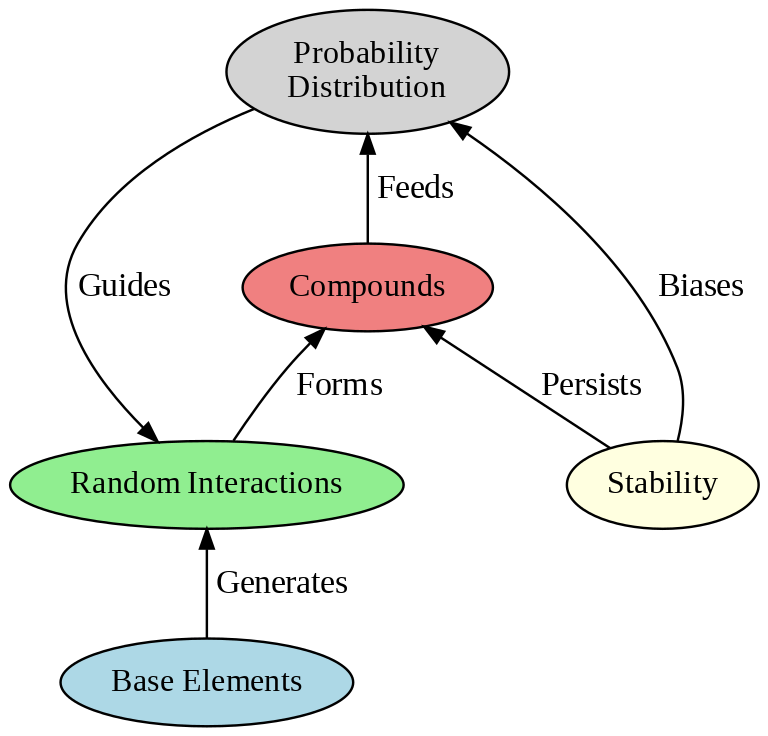
\includegraphics[width=0.6\textwidth]{SDA-top-down.png}
    \caption{Feedback structure underlying chemical SDA dynamics. Base elements interact randomly to form compounds. Compounds that persist contribute more to the population, biasing the probability distribution. This distribution in turn guides future interactions, closing a feedback loop. The result is emergent roulette-wheel selection.}
    \label{fig:top-down}
\end{figure}

The feedback structure shown in Figure~\ref{fig:top-down} provides a mechanistic explanation for how GA-like search emerges spontaneously in chemical SDA. In conventional genetic algorithms, roulette-wheel selection is imposed externally: the algorithm samples parents in proportion to a user-defined fitness function. In SDA, no such programmer is required. Instead, stability imbalances ensure that some compounds persist longer than others. Persistence in turn biases the probability distribution over the population, which then guides future interactions. 

This feedback loop closes the causal chain: compounds shape the distribution, the distribution shapes sampling, and sampling determines which compounds are likely to appear again. In effect, selection pressure is not imposed top–down but emerges bottom–up from persistence differences within the population. The result is indistinguishable in practice from roulette-wheel selection, yet it arises naturally from the dynamics of the system.

This perspective also clarifies the often-misused notion of “top-down causation.” There is no need to posit a mystical programmer or abstract force directing the search. What appears as top–down influence of the probability distribution on individual elements is mechanistically explained by the accumulation of persistence imbalances at the population level. Stability alone suffices to generate the feedback necessary for open-ended, GA-like evolution.



\section{Discussion and Implications}

\subsection{Open-Endedness and Computation}
SDA can be understood as a Markov process on an effectively infinite state space. 
Unlike equilibrium models that converge to fixed points, the SDA dynamics continually 
expand the accessible state space by recombination and mutation. In this sense, 
Kauffman’s “adjacent possible” becomes quantifiable: each generation explores a 
countable, probabilistic frontier of assemblies. The search is the optimization, 
with no prespecified target.  

This perspective connects SDA to computation. Just as genetic programming 
demonstrated that variation, selection, and recombination can evolve nontrivial 
algorithms, SDA suggests that matter itself can evolve universal computation. 
In Lloyd’s view, the universe computes bottom–up via bit flips governed by 
physical laws. SDA, in contrast, represents a self-modifying computation driven 
by a feedback loop between persistence landscapes and assembly dynamics, 
generative rather than merely simulative.  

\subsection{The Evolutionary Ladder}  
The SDA/GA perspective helps to situate chemical evolution within a broader ladder of dynamical processes that may bridge chemistry and biology. At the base lies \textit{persistence}: some motifs survive longer than others. Persistence enables \textit{catalysis}, where stable motifs influence the production rates of other compounds. With further reinforcement, \textit{autocatalysis} arises, as motifs begin to promote their own formation. Only at a higher rung does \textit{replication} appear, once templating and copying mechanisms become possible. Beyond replication, motifs can acquire specific \textit{functions} in metabolic or structural roles, eventually coalescing into the integrated networks characteristic of \textit{biology}.  

This framing highlights that replication is not the foundation of evolution but one rung in a continuum that begins with persistence and extends upward through catalysis, autocatalysis, and functional integration. The chemical SDA simulations correspond to the earliest stages, demonstrating that persistence imbalances alone are sufficient to initiate evolutionary dynamics.  

\subsection{Echoes in Biology}  

The principle of persistence-driven selection does not end with chemistry but recurs at multiple levels of biological organization. At the genetic level, \textit{selfish elements} such as transposons and introns propagate not because they enhance organismal fitness, but because they persist in genomic lineages long enough to bias inheritance. Similarly, \textit{codon usage bias} reflects stability effects in translational dynamics: codons that are more robust to errors or that align with abundant tRNAs persist more readily, shaping the genetic code over evolutionary time.  

At the level of organisms and populations, persistence manifests in traits such as longevity and life-history strategies. Price’s equation formalizes how traits that extend survival beyond reproductive years can bias the survival and reproduction of others, aligning with SDA’s emphasis on persistence as a population-level driver. Longevity may therefore act as a scaffold for cultural transmission, cooperative behavior, and catalytic roles in social or ecological systems, much as stable motifs scaffold chemical innovations. Keystone species provide a parallel ecological example, since their persistence stabilizes entire communities and reshapes the probability landscape for other species.  

In each of these contexts, persistence skews the distribution of possibilities, creating emergent selection without an external programmer. The same feedback loop of stability leading to persistence, persistence leading to population skew, and skew biasing future interactions recurs across scales from molecules to ecosystems. These echoes suggest that the mechanisms demonstrated in chemical simulations reflect a more general evolutionary logic embedded in natural systems.



\section{Conclusions}

This work has advanced \textit{Stability-Driven Assembly} (SDA) as a concrete mechanism by which selection-like dynamics can emerge in the absence of explicit fitness functions or dedicated replicators. The core mechanism is simple: persistence imbalances skew the population, and that skew feeds back to parent sampling so that longer-lived motifs are chosen more often for subsequent interactions. In expectation, this implements the equivalent of roulette–wheel selection. Thus, the loop \emph{create $\rightarrow$ persist $\rightarrow$ sample} constitutes a natural genetic algorithm (SDA/GA), with stability playing the role of fitness supplied by the environment rather than by a programmer.

The chemical instantiation demonstrates this mechanism in practice. Final-population histograms show oligopolistic dominance by a few scaffolds; the two–motif evolution analysis reveals schema competition and eventual convergence to a highly persistent scaffold family; entropy and diversity traces exhibit early expansion followed by consolidation; and the final rank–abundance curve is heavy–tailed, with a small number of winners and a long tail of rare species. Together, these observations are the characteristic signatures of selection acting on a generative process: novelty is continually produced, but long-term residence time determines which motifs accumulate.

These results stand in contrast to equilibrium analyses (e.g., constant–rate, well–mixed models in the spirit of MAK), which are linearized to ensure mathematical tractability and therefore tend to suppress the very feedbacks that drive open-ended evolution. In SDA/GA, effective rates are nonuniform because stability differs across motifs; persistence imbalances bias the population and hence future sampling. What appears as a steady state in equilibrium settings is, in SDA/GA, the moving target of an evolving distribution shaped by selection, turnover, and replacement.

\subsection{Limitations}
Our implementation deliberately isolates the population–level mechanism and makes several simplifying assumptions. The stability function $S(p)$ is heuristic rather than derived from first–principles thermodynamics or explicit kinetics; operators (recombination and single–site mutation) abstract multi–step synthesis pathways; the system is effectively well–mixed with constant replenishment; and explicit solvent effects, transport, and residence–time distributions are not modeled. These simplifications are appropriate for clarifying mechanism but limit quantitative interpretation.

\subsection{Future Work}

Several extensions follow naturally from this work. A first direction is to conduct multi-run statistical analyses, quantifying variability across independent trials with identical hyperparameters and testing sensitivity to parameters such as interaction count, replenishment rate, mutation probability, and initial seed. A second avenue is to enrich the stability function $S(p)$ beyond the current heuristic formulation, grounding it in more realistic physical and chemical principles. Candidate approaches include semiempirical or DFT-based energy estimates, incorporation of activation barriers and solvent corrections, and microkinetic models that incorporate residence-time distributions.  

Chemically, the model can be expanded to include additional classes of reactions beyond simple recombination and mutation. Acid–base cycles, isomerization kinetics, polymerization with chain-length and end-group effects, as well as dissociation and reversible transformations, would all allow a more faithful mapping between the SDA operators and real chemical processes. Complementing these theoretical extensions, an experimental roadmap can be envisioned: an open, driven reactor system with periodic feed–flush cycles, controlled energy or catalyst inputs, and continuous monitoring through MS, LC–MS, or NMR could directly measure abundance skew, entropy and diversity trajectories, and scaffold turnover. Such experiments would allow calibration of $S(p)$ against observed lifetimes and persistence data.  


\subsection{Information as an Evolving Property}

The SDA/GA perspective suggests a restrained but important claim about information: it is not a prerequisite substance imposed on matter, but an \emph{emergent property of population dynamics} shaped by persistence and stochastic creation. As distributions become skewed by stability, structured regularities accumulate and are propagated by the very feedback that produced them. In this sense (and as argued more generally in our prior work), information arises from the coupling of generative processes with selection pressures, rather than from an externally specified target.

In sum, SDA/GA provides a minimal, mechanistic pathway by which chemistry can exhibit evolutionary search: stability differences induce population skew; skew induces effective selection; and selection, coupled to ongoing creation, yields both novelty and order. By grounding this loop in chemical symbol space, we have shown how a natural genetic algorithm can emerge from persistence alone, and we have outlined concrete experimental and theoretical steps to test, refine, and extend this framework.

\section{Simulation Code}

All Python code and simulation results are openly available at:
\url{https://github.com/danadler-dev/MDPI-Life-Article}. 
The repository README includes a link to an interactive Google Colab notebook  with the complete code and outputs corresponding to the figures and experiments presented in this paper.

\begin{adjustwidth}{-\extralength}{0cm}
%\printendnotes[custom] % Un-comment to print a list of endnotes

\reftitle{References}



% Please provide either the correct journal abbreviation (e.g. according to the “List of Title Word Abbreviations” http://www.issn.org/services/online-services/access-to-the-ltwa/) or the full name of the journal.
% Citations and References in Supplementary files are permitted provided that they also appear in the reference list here. 

%=====================================
% References, variant A: external bibliography
%=====================================
% \bibliography{your_external_BibTeX_file}

%=====================================
% References, variant B: internal bibliography
%=====================================

% ACS format
\isAPAandChicago{}{%
\begin{thebibliography}{999}
% Reference 1

\bibitem{kauffman1995home}
Kauffman, S. \textit{At Home in the Universe: The Search for the Laws of Self-Organization and Complexity}; Oxford University Press: New York, NY, USA, 1995.

\bibitem{fisher1930genetical}
Fisher, R.A. \textit{The Genetical Theory of Natural Selection}; Oxford University Press: Oxford, UK, 1930.

\bibitem{davies2006goldilocks}
Davies, P. \textit{The Goldilocks Enigma: Why is the Universe Just Right for Life?}; Allen Lane: London, UK, 2006.

\bibitem{hordijk2012autocatalytic}
Hordijk, W.; Steel, M.; Kauffman, S. \textit{The Structure of Autocatalytic Sets: Evolvability, Enablement, and Emergence.} Acta Biotheoretica \textbf{2012}, \textit{60}, 379–392.

\bibitem{nghe2015prebiotic}
Nghe, P.; Hordijk, W.; Kauffman, S.A.; Walker, S.I.; Schmidt, F.J.; Kemble, H.; Yeates, J.A.; Lehman, N. \textit{Prebiotic network evolution: Six key parameters.} Molecular BioSystems \textbf{2015}, \textit{11}, 3206–3217.

\bibitem{kolmogorov1965complexity}
Kolmogorov, A.N. \textit{Three Approaches to the Quantitative Definition of Information.} Problemy Peredachi Informatsii \textbf{1965}, \textit{1}, 3–11.

\bibitem{chaitin1977algorithmic}
Chaitin, G.J. \textit{Algorithmic Information Theory.} IBM J. Res. Dev. \textbf{1977}, \textit{21}, 350–359.

\bibitem{solomonoff1964formal}
Solomonoff, R.J. \textit{A Formal Theory of Inductive Inference. Part I and Part II.} Inf. Control \textbf{1964}, \textit{7}, 1–22, 224–254.

\bibitem{shannon1948mathematical}
Shannon, C.E. \textit{A Mathematical Theory of Communication.} Bell Syst. Tech. J. \textbf{1948}, \textit{27}, 379–423.

\bibitem{deutsch2013constructor}
Deutsch, D.; Marletto, C. \textit{Constructor theory of information.} Proceedings of the Royal Society A: Mathematical, Physical and Engineering Sciences \textbf{2015}, \textit{471}, 20140540.

\bibitem{walker2023nature}
Walker, S.I.; Cronin, L.; et al. \textit{Assembly theory explains and quantifies selection and evolution across physical and biological systems.} Nature \textbf{2023}, \textit{618}, 619-628.

\bibitem{schrodinger1944life}
Schrödinger, E. \textit{What is Life?}; Cambridge University Press: Cambridge, UK, 1944.

\bibitem{pross2016life}
Pross, A. \textit{What is Life? How Chemistry Becomes Biology}; Oxford University Press: Oxford, UK, 2016.

\bibitem{kauffman1986autocatalytic}
Kauffman, S.A. \textit{Autocatalytic sets of proteins.} Journal of Theoretical Biology \textbf{1986}, \textit{119}, 1–24.

\bibitem{hordijk2011required}
Hordijk, W.; Kauffman, S.A.; Steel, M. \textit{Required levels of catalysis for emergence of autocatalytic sets in models of chemical reaction systems.} International Journal of Molecular Sciences \textbf{2011}, \textit{12}, 3085–3101.

\bibitem{eigen}
Eigen M. \textit{The Hypercycle: A Principle of Natural Self-Organization.} Springer, 1979.

\bibitem{fontana1991algorithmic}
Fontana, W. \textit{Algorithmic chemistry.} Artificial Life II \textbf{1991}, \textit{11}, 159–209.

\bibitem{cronin2024chemputation}
Cronin, L.; Pagel, S.; Sharma, A. \textit{The Chemputer and Chemputation: A Universal Chemical Compound Synthesis Machine}. Preprint available on arXiv (August 2024), arXiv:2408.09171.

\bibitem{barabasi1999emergence}
Barabási, A.-L.; Albert, R. \textit{Emergence of Scaling in Random Networks.} Science \textbf{1999}, \textit{286}, 509–512.

\bibitem{nowak2006evolutionary}
Nowak, M.A. \textit{Evolutionary Dynamics: Exploring the Equations of Life}; Belknap Press: Cambridge, MA, USA, 2006.

\bibitem{england2015dissipative}
England, J.L. \textit{Dissipative Adaptation in Driven Self-Assembly.} Nature Nanotechnology \textbf{2015}, \textit{10}, 919–923.

\bibitem{wu2012origin}
Wu, M.; Higgs, P.G. \textit{Origin of self-replicating biopolymers: Autocatalytic feedback can trump power law replication.} Journal of Molecular Evolution \textbf{2012}, \textit{74}, 91–102.

\bibitem{prigogine1977self}
Prigogine, I.; Nicolis, G. \textit{Self-Organization in Non-Equilibrium Systems}; Wiley: New York, NY, USA, 1977.

\bibitem{nicolis1977self}
Nicolis, G.; Prigogine, I. \textit{Self-Organization in Nonequilibrium Systems: From Dissipative Structures to Order through Fluctuations}; Wiley: New York, NY, USA, 1977.

\bibitem{noble2012causality}
Noble, D. \textit{A Theory of Biological Relativity: No Privileged Level of Causation.} Interface Focus \textbf{2012}, \textit{2}, 55–64.

\bibitem{gardiner2009} Gardiner, C. W. (2009). \textit{Stochastic Methods: A Handbook for the Natural and Social Sciences} (4th ed.). Springer.

\bibitem{adler_sda}
Adler, D.
\textit{Stability-Driven Assembly Theory}.
SSRN Preprint, 2025. Available at: \url{https://dx.doi.org/10.2139/ssrn.5203036}

\bibitem{holland1975adaptation}
Holland, J.H. \textit{Adaptation in Natural and Artificial Systems}; University of Michigan Press: Ann Arbor, MI, USA, 1975.

\bibitem{goldberg1989genetic}
Goldberg, D.E. \textit{Genetic Algorithms in Search, Optimization, and Machine Learning}; Addison-Wesley: Boston, MA, USA, 1989.

\bibitem{koza1992genetic}
Koza, J. R.
\textit{Genetic Programming: On the Programming of Computers by Means of Natural Selection}.
MIT Press, Cambridge, MA, USA, 1992.

\bibitem{adler1993marriage}
Adler, D. \textit{Genetic algorithms and simulated annealing: a marriage proposal}. Proceedings of the IEEE International Conference on Neural Networks, San Francisco, CA, USA, 1993; pp. 1759--1764. doi:10.1109/ICNN.1993.298712.

\bibitem{segre2000compositional}
Segre, D.; Ben-Eli, D.; Lancet, D. \textit{Compositional genomes: Prebiotic information transfer in mutually catalytic noncovalent assemblies}. Proc. Natl. Acad. Sci. USA \textbf{2000}, 97, 4112--4117.

\bibitem{markovitch2012universal}
Markovitch, O.; Lancet, D. \textit{Excess mutual catalysis is required for effective evolvability}. Artif. Life \textbf{2012}, 18, 243--266.

\bibitem{hordijk2012autocatalytic}
Hordijk, W.; Steel, M.; Kauffman, S. \textit{The structure of autocatalytic sets: Evolvability, enablement, and emergence}. J. Theor. Biol. \textbf{2012}, 295, 1--16.

\bibitem{adami2000avida}
Adami, C. \textit{Introduction to artificial life}. Springer: New York, NY, USA, 1998.

\bibitem{ray1992tierra}
Ray, T.S. \textit{An approach to the synthesis of life}. Artificial Life II \textbf{1992}, 371--408.

\bibitem{damer2015coupled}
Damer, B.; Deamer, D. \textit{Coupled phases and combinatorial selection in fluctuating hydrothermal pools: A scenario to guide experimental approaches to the origin of cellular life}. Astrobiology \textbf{2015}, 15, 861--877.


\bibitem{dawkins1986blind}
Dawkins, R. \textit{The Blind Watchmaker}; W.W. Norton: New York, NY, USA, 1986.

\bibitem{adler2025jazz}
Adler, D. \textit{Active Listening in Jazz}. Available online: \url{https://jazzintro.com}.

\bibitem{fink2007gdb11}
Fink, T.; Reymond, J.-L.
\textit{Virtual exploration of the chemical universe up to 11 atoms of C, N, O, F:
Assembly of 26.4 million structures (GDB-11).}
J. Chem. Inf. Model. 2007, 47, 342--353.

\bibitem{brown2004ga}
Brown, N.; McKay, B.; Gilardoni, F.; Gasteiger, J.
\textit{A graph-based genetic algorithm and its application to the multiobjective
evolution of median molecules.}
J. Chem. Inf. Comput. Sci. 2004, 44, 1079--1087.

\bibitem{lewis1998gp}
Lewis, R. A.
\textit{Genetic programming as a model for drug design.}
J. Chem. Inf. Comput. Sci. 1998, 38, 651--657.

\bibitem{jensen2019ga}
Jensen, J. H.
\textit{A graph-based genetic algorithm and generative model/GA hybrid for molecular discovery.}
Chem. Sci. 2019, 10, 3567--3572.

\bibitem{yoshikawa2018ga}
Yoshikawa, N.; Terayama, K.; Sumita, M.; Homma, T.; Oono, K.; Tsuda, K.
\textit{Population-based de novo molecule generation, using grammatical evolution.}
Chem. Lett. 2018, 47, 1431--1434.

\bibitem{landrum2006rdkit}
Landrum, G. (2006). \textit{RDKit: Open-source cheminformatics}. Available at: \url{http://www.rdkit.org}.

\bibitem{degen2008art}
Degen, J., Wegscheid-Gerlach, C., Zaliani, A., Rarey, M. (2008).
\textit{On the art of compiling and using ‘drug-like’ chemical fragment spaces}.
\textit{ChemMedChem}, 3(10), 1503–1507. https://doi.org/10.1002/cmdc.200800178

\bibitem{janet2023bestpractices}
Janet, J. P., Duan, C., Yang, T., Kulik, H. J. (2023).
\textit{Determining best practices for using genetic algorithms in molecular discovery}.
\textit{Journal of Chemical Physics}, 159(9), 091501. https://doi.org/10.1063/5.0158336


\end{thebibliography}
}



% If authors have biography, please use the format below
%\section*{Short Biography of Authors}
%\bio
%{\raisebox{-0.35cm}{\includegraphics[width=3.5cm,height=5.3cm,clip,keepaspectratio]{Definitions/author1.pdf}}}
%{\textbf{Firstname Lastname} Biography of first author}
%
%\bio
%{\raisebox{-0.35cm}{\includegraphics[width=3.5cm,height=5.3cm,clip,keepaspectratio]{Definitions/author2.jpg}}}
%{\textbf{Firstname Lastname} Biography of second author}

% For the MDPI journals use author-date citation, please follow the formatting guidelines on http://www.mdpi.com/authors/references
% To cite two works by the same author: \citeauthor{ref-journal-1a} (\citeyear{ref-journal-1a}, \citeyear{ref-journal-1b}). This produces: Whittaker (1967, 1975)
% To cite two works by the same author with specific pages: \citeauthor{ref-journal-3a} (\citeyear{ref-journal-3a}, p. 328; \citeyear{ref-journal-3b}, p.475). This produces: Wong (1999, p. 328; 2000, p. 475)

%%%%%%%%%%%%%%%%%%%%%%%%%%%%%%%%%%%%%%%%%%
%% for journal Sci
%\reviewreports{\\
%Reviewer 1 comments and authors’ response\\
%Reviewer 2 comments and authors’ response\\
%Reviewer 3 comments and authors’ response
%}
%%%%%%%%%%%%%%%%%%%%%%%%%%%%%%%%%%%%%%%%%%
\PublishersNote{}
%\isPreprints{} % If the paper is ``preprints'', please uncomment this parenthesis.
\end{document}

